\documentclass[12pt]{article}

\usepackage{hcmus-report-template}

\usepackage{graphicx}
\usepackage{float}
\usepackage{placeins}
\usepackage{dirtree}
\usepackage{tabularx}
\usepackage{booktabs}
\usepackage{multirow}
\usepackage{enumitem}
\usepackage{tikz}
\usetikzlibrary{shapes.geometric, arrows.meta, positioning}

% Disable indentation on new paragraphs
\setlength{\parindent}{0pt}

% Line spacing 1.5
\renewcommand{\baselinestretch}{1.5}

% Graphic path
\graphicspath{{img/}}

% To use Times font family, uncomment this row
% \usepackage{mathptmx}

% To use roman section / subsection, uncomment these rows
% \renewcommand{\thesection}{\Roman{section}}
% \renewcommand{\thesubsection}{\thesection.\Roman{subsection}}

% Define course name, report name and report title.
\newcommand{\coursename}{CSC17001 - Phân tích dữ liệu thông minh}
\newcommand{\reportname}{Exploring Mental Health}
\newcommand{\reporttitle}{BÁO CÁO ĐỒ ÁN THỰC HÀNH}

\newcommand{\studentname}{Trần Hữu Kim Thành - 23120166 \\ Đàm Tiến Đạt - 23120118 \\ Triệu Tuấn Kiệt - 23120137 \\ Lê Nhật Minh Tâm - 23120163 \\ Nguyễn Hồ Anh Tuấn - 23120185}
\newcommand{\teachername}{Thầy Nguyễn Thanh Tình}

% Header
\lhead{\reporttitle}
\rhead{
Trường Đại học Khoa học Tự nhiên - ĐHQG HCM\\
\coursename
}

% Footer


% ============ DOCUMENT ============
\begin{document}

\pagenumbering{roman}
\input{content/title}

\cleardoublepage
\pagenumbering{roman}
\pagestyle{empty} 

\tableofcontents
\cleardoublepage

\listoffigures
\cleardoublepage

\listoftables
\cleardoublepage

\pagenumbering{arabic} 
\pagestyle{plain}
      
\setcounter{page}{1}

\section{Phân công công việc}
\label{sec:planning}

Dự án được thực hiện bởi nhóm 5 thành viên. Bảng~\ref{tab:task_distribution} trình bày chi tiết phân công nhiệm vụ và tỷ lệ đóng góp của từng thành viên. Điểm cá nhân được tính theo công thức:

\begin{equation}
\text{Điểm cá nhân} = \text{Điểm nhóm} \times \text{\% Đóng góp}
\label{eq:individual_score}
\end{equation}

\begin{table}[H]
\centering
\caption{Bảng phân công nhiệm vụ và đánh giá đóng góp}
\label{tab:task_distribution}
\begin{tabular}{clp{7cm}c}
\toprule
\textbf{STT} & \textbf{Họ tên — MSSV} & \textbf{Nhiệm vụ} & \textbf{\% Đóng góp} \\
\midrule
1 & Trần Hữu Kim Thành — 23120166 & NB1, NB6, Kiểm tra và sửa các NB, Báo cáo LaTeX & 100\% \\
2 & Đàm Tiến Đạt — 23120118 & NB3, Báo cáo LaTeX & 100\% \\
3 & Triệu Tuấn Kiệt — 23120137 & NB2, Báo cáo LaTeX & 100\% \\
4 & Lê Nhật Minh Tâm — 23120163 & NB5, Báo cáo LaTeX, Edit Video & 100\% \\
5 & Nguyễn Hồ Anh Tuấn — 23120185 & NB4, Báo cáo LaTeX, Edit Video & 100\% \\
\bottomrule
\end{tabular}
\end{table}

\textbf{Link video thuyết trình}: \url{https://www.youtube.com/watch?v=TODO}

\section{Tổng quan dự án}
\label{sec:overview}

\subsection{Giới thiệu bài toán}

Dự án này được lấy cảm hứng từ cuộc thi Kaggle \textit{``Playground Series --- Season 4, Episode 11: Exploring Mental Health Data''}~\cite{kaggle2024}. Mục tiêu chính là xây dựng mô hình học máy để dự đoán liệu một cá nhân có nguy cơ bị trầm cảm (\textit{Depression}) hay không, dựa trên dữ liệu khảo sát sức khỏe tâm thần.

\textbf{Phát biểu bài toán:} Cho trước một tập dữ liệu gồm các đặc trưng nhân khẩu học, học vấn, nghề nghiệp và các yếu tố tâm lý --- xã hội, bài toán yêu cầu phân loại nhị phân (\textit{Binary Classification}) để dự đoán biến mục tiêu \texttt{Depression} nhận giá trị 0 (không trầm cảm) hoặc 1 (trầm cảm).

\subsection{Mô tả dữ liệu}

Bộ dữ liệu được cung cấp bởi Kaggle với các thông tin chính:

\begin{itemize}[noitemsep]
    \item \textbf{Tập huấn luyện (train)}: 140.700 mẫu với 20 đặc trưng và 1 biến mục tiêu
    \item \textbf{Tập kiểm tra (test)}: 93.800 mẫu (không có nhãn)
    \item \textbf{Tính chất}: Dữ liệu tổng hợp (\textit{synthetic}), được tạo từ mô hình deep learning huấn luyện trên dữ liệu khảo sát thực tế
    \item \textbf{Metric đánh giá}: Accuracy (theo yêu cầu cuộc thi)
\end{itemize}

\subsection{Pipeline tổng thể}

Hình~\ref{fig:pipeline} minh họa toàn bộ quy trình xử lý dữ liệu và xây dựng mô hình của dự án, bao gồm 6 giai đoạn chính từ dữ liệu thô đến kết quả dự đoán cuối cùng.

\begin{figure}[H]
\centering
\begin{tikzpicture}[
    node distance=1.2cm,
    block/.style={rectangle, rounded corners, draw=black!70, fill=blue!8,
                  text width=3.2cm, minimum height=1cm, align=center, font=\small\bfseries},
    arrow/.style={-{Stealth[length=3mm]}, thick, draw=black!60}
]
\node[block] (raw) {1. Dữ liệu thô\\(Raw Data)};
\node[block, right=of raw] (eda) {2. Khám phá\\dữ liệu (EDA)};
\node[block, right=of eda] (prep) {3. Tiền xử lý\\(Preprocessing)};
\node[block, below=of prep] (fe) {4. Kỹ thuật\\đặc trưng (FE)};
\node[block, left=of fe] (model) {5. Xây dựng\\mô hình};
\node[block, left=of model] (eval) {6. Đánh giá\\(Evaluation)};

\draw[arrow] (raw) -- (eda);
\draw[arrow] (eda) -- (prep);
\draw[arrow] (prep) -- (fe);
\draw[arrow] (fe) -- (model);
\draw[arrow] (model) -- (eval);
\end{tikzpicture}
\caption{Pipeline tổng thể của dự án dự đoán rủi ro trầm cảm}
\label{fig:pipeline}
\end{figure}

\section{Khám phá dữ liệu (EDA)}
\label{sec:eda}

\subsection{Tổng quan Dataset}
\label{subsec:dataset_overview}

Bộ dữ liệu bao gồm 140.700 mẫu huấn luyện và 93.800 mẫu kiểm tra với 20 đặc trưng đầu vào. Bảng~\ref{tab:features} trình bày danh sách các đặc trưng cùng kiểu dữ liệu và ý nghĩa tương ứng.

\begin{table}[H]
\centering
\caption{Danh sách các đặc trưng trong bộ dữ liệu}
\label{tab:features}
\small
\begin{tabular}{llp{7.5cm}}
\toprule
\textbf{Tên đặc trưng} & \textbf{Kiểu} & \textbf{Ý nghĩa} \\
\midrule
Name & Text & Tên người tham gia khảo sát \\
Age & Numerical & Tuổi \\
Gender & Categorical & Giới tính (Male / Female) \\
City & Categorical & Thành phố sinh sống \\
Working Professional or Student & Categorical & Đang đi làm hay sinh viên \\
Profession & Categorical & Nghề nghiệp \\
Degree & Categorical & Trình độ học vấn \\
Academic Pressure & Numerical & Áp lực học tập (1--5) \\
Work Pressure & Numerical & Áp lực công việc (1--5) \\
CGPA & Numerical & Điểm trung bình tích lũy \\
Study Satisfaction & Numerical & Mức hài lòng với việc học (1--5) \\
Job Satisfaction & Numerical & Mức hài lòng với công việc (1--5) \\
Sleep Duration & Categorical & Thời lượng ngủ \\
Dietary Habits & Categorical & Thói quen ăn uống \\
Have you ever had suicidal thoughts? & Binary & Từng có suy nghĩ tự tử \\
Work/Study Hours & Numerical & Số giờ làm việc / học mỗi ngày \\
Financial Stress & Numerical & Mức độ căng thẳng tài chính (1--5) \\
Family History of Mental Illness & Binary & Gia đình có tiền sử bệnh tâm thần \\
\midrule
\textbf{Depression} & \textbf{Binary} & \textbf{Biến mục tiêu: 0 = Không, 1 = Có} \\
\bottomrule
\end{tabular}
\end{table}

\subsection{Phân tích biến mục tiêu}
\label{subsec:target_analysis}

Hình~\ref{fig:target_dist} cho thấy phân phối của biến mục tiêu \texttt{Depression}. Tập dữ liệu có sự mất cân bằng đáng kể: 115.133 mẫu thuộc lớp 0 (không trầm cảm, chiếm 81,8\%) và 25.567 mẫu thuộc lớp 1 (trầm cảm, chiếm 18,2\%). Tỷ lệ mất cân bằng xấp xỉ 4,5:1, đây là mức mất cân bằng vừa phải (\textit{moderate imbalance}) và cần được lưu ý trong quá trình huấn luyện mô hình.

\begin{figure}[H]
\centering
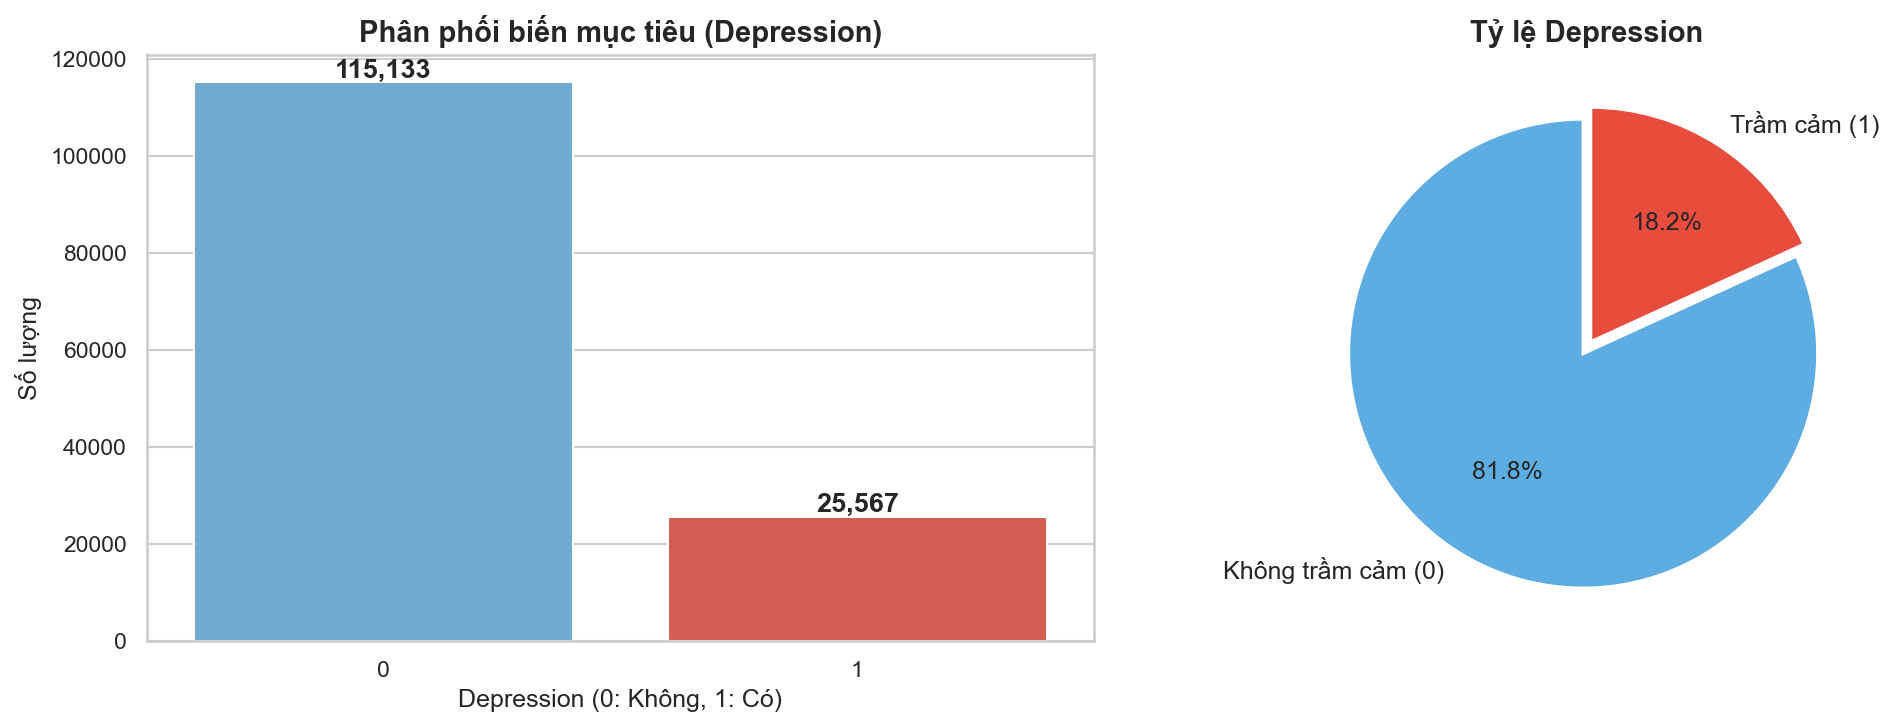
\includegraphics[width=0.95\textwidth]{eda/target_distribution.png}
\caption{Phân phối biến mục tiêu Depression: biểu đồ cột (trái) và biểu đồ tròn (phải)}
\label{fig:target_dist}
\end{figure}

\subsection{Phân tích đặc trưng --- Bivariate Analysis}
\label{subsec:bivariate}

Để hiểu mối quan hệ giữa từng đặc trưng với biến mục tiêu, nhóm tác giả tiến hành phân tích hai biến (\textit{bivariate analysis}) cho các đặc trưng quan trọng nhất.

\textbf{Age vs Depression} (Hình~\ref{fig:age_vs_dep}): Tuổi là đặc trưng có tương quan mạnh nhất với Depression ($r = -0,565$). Nhóm tuổi trẻ (18--30) có tỷ lệ trầm cảm cao hơn rõ rệt so với nhóm tuổi lớn hơn. Phân phối KDE cho thấy sự phân tách rõ ràng giữa hai lớp: nhóm trầm cảm tập trung ở độ tuổi 20--30, trong khi nhóm không trầm cảm phân bố đều hơn.

\begin{figure}[H]
\centering
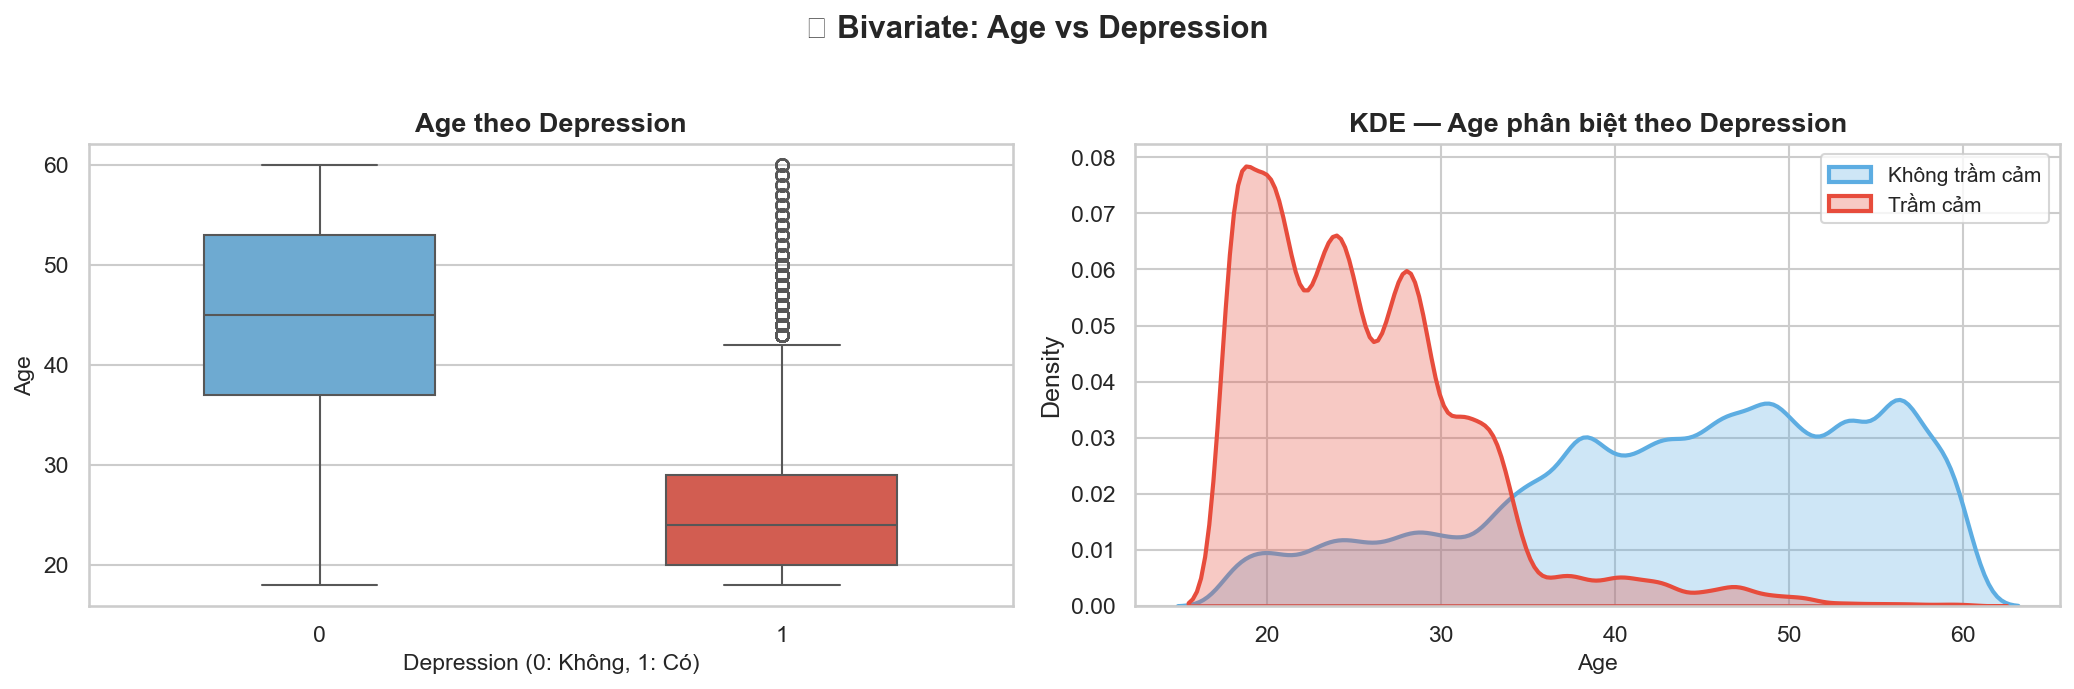
\includegraphics[width=0.95\textwidth]{eda/plot_numerical_vs_target_Age.png}
\caption{Phân tích Age vs Depression: boxplot (trái) và KDE (phải)}
\label{fig:age_vs_dep}
\end{figure}

\textbf{Academic Pressure vs Depression} (Hình~\ref{fig:acad_vs_dep}): Áp lực học tập có tương quan dương mạnh với Depression ($r = 0,475$). Nhóm trầm cảm có median Academic Pressure = 4, trong khi nhóm không trầm cảm có median = 2. Phân phối KDE minh họa rõ: nhóm không trầm cảm tập trung ở mức thấp (1--2), nhóm trầm cảm thiên về mức cao (4--5).

\begin{figure}[H]
\centering
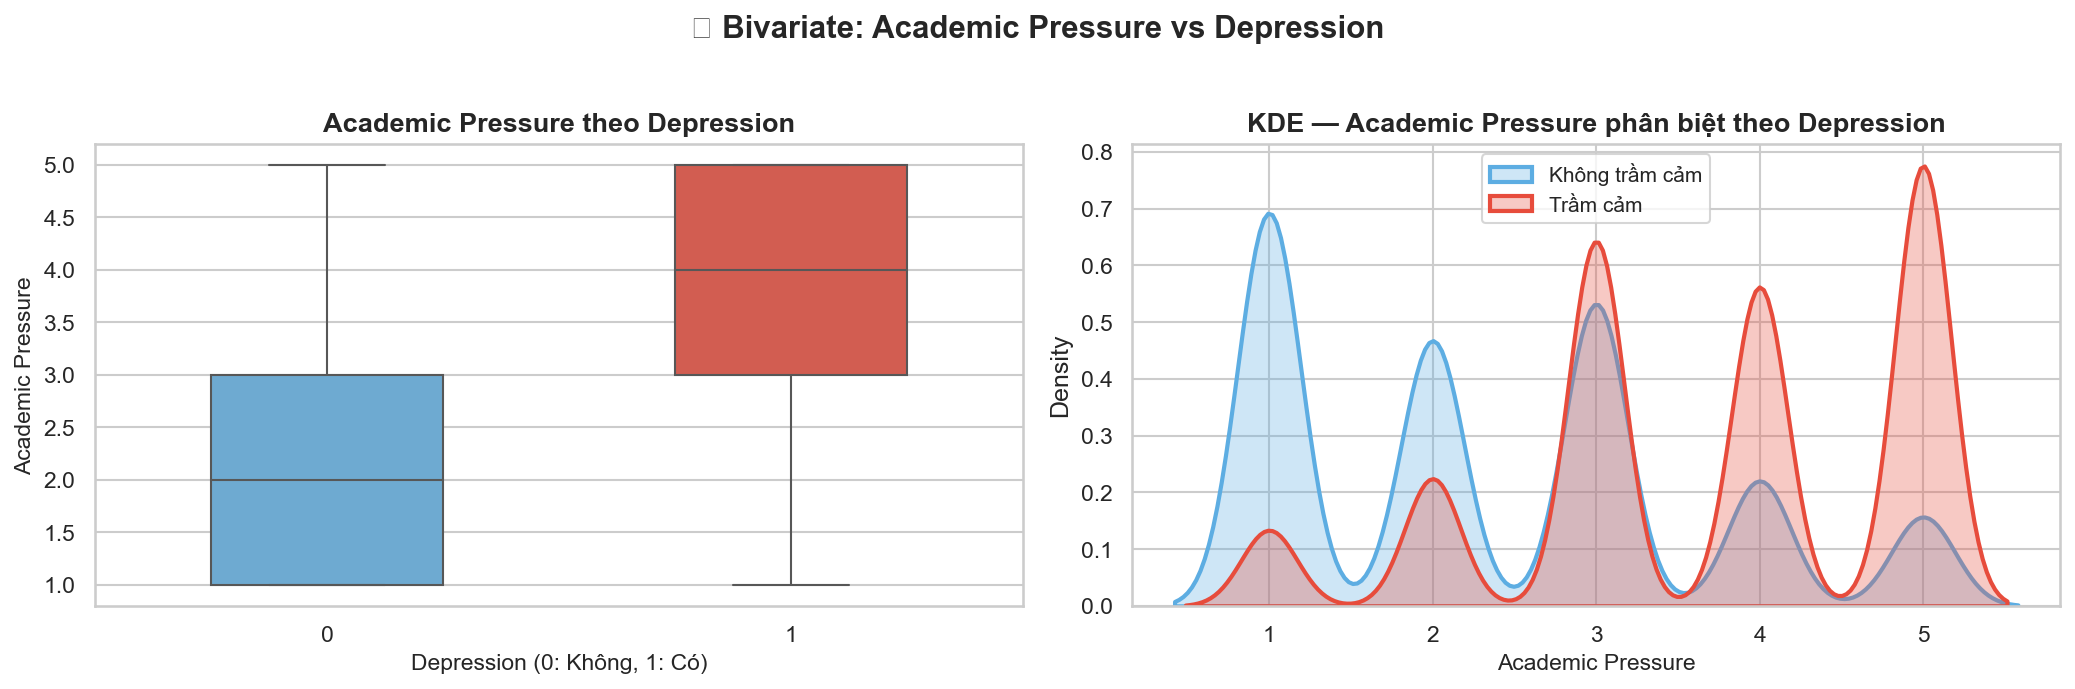
\includegraphics[width=0.95\textwidth]{eda/plot_numerical_vs_target_Academic_Pressure.png}
\caption{Phân tích Academic Pressure vs Depression: boxplot (trái) và KDE (phải)}
\label{fig:acad_vs_dep}
\end{figure}

\textbf{Suicidal Thoughts vs Depression} (Hình~\ref{fig:suicidal_vs_dep}): Đây là đặc trưng nhị phân có khả năng phân biệt mạnh nhất. Trong nhóm từng có suy nghĩ tự tử, tỷ lệ trầm cảm là 31,8\%, cao gấp 6,5 lần so với nhóm chưa từng (4,9\%). Kết quả này phù hợp với kiến thức y học: suy nghĩ tự tử là một trong những dấu hiệu cảnh báo quan trọng nhất của trầm cảm.

\begin{figure}[H]
\centering
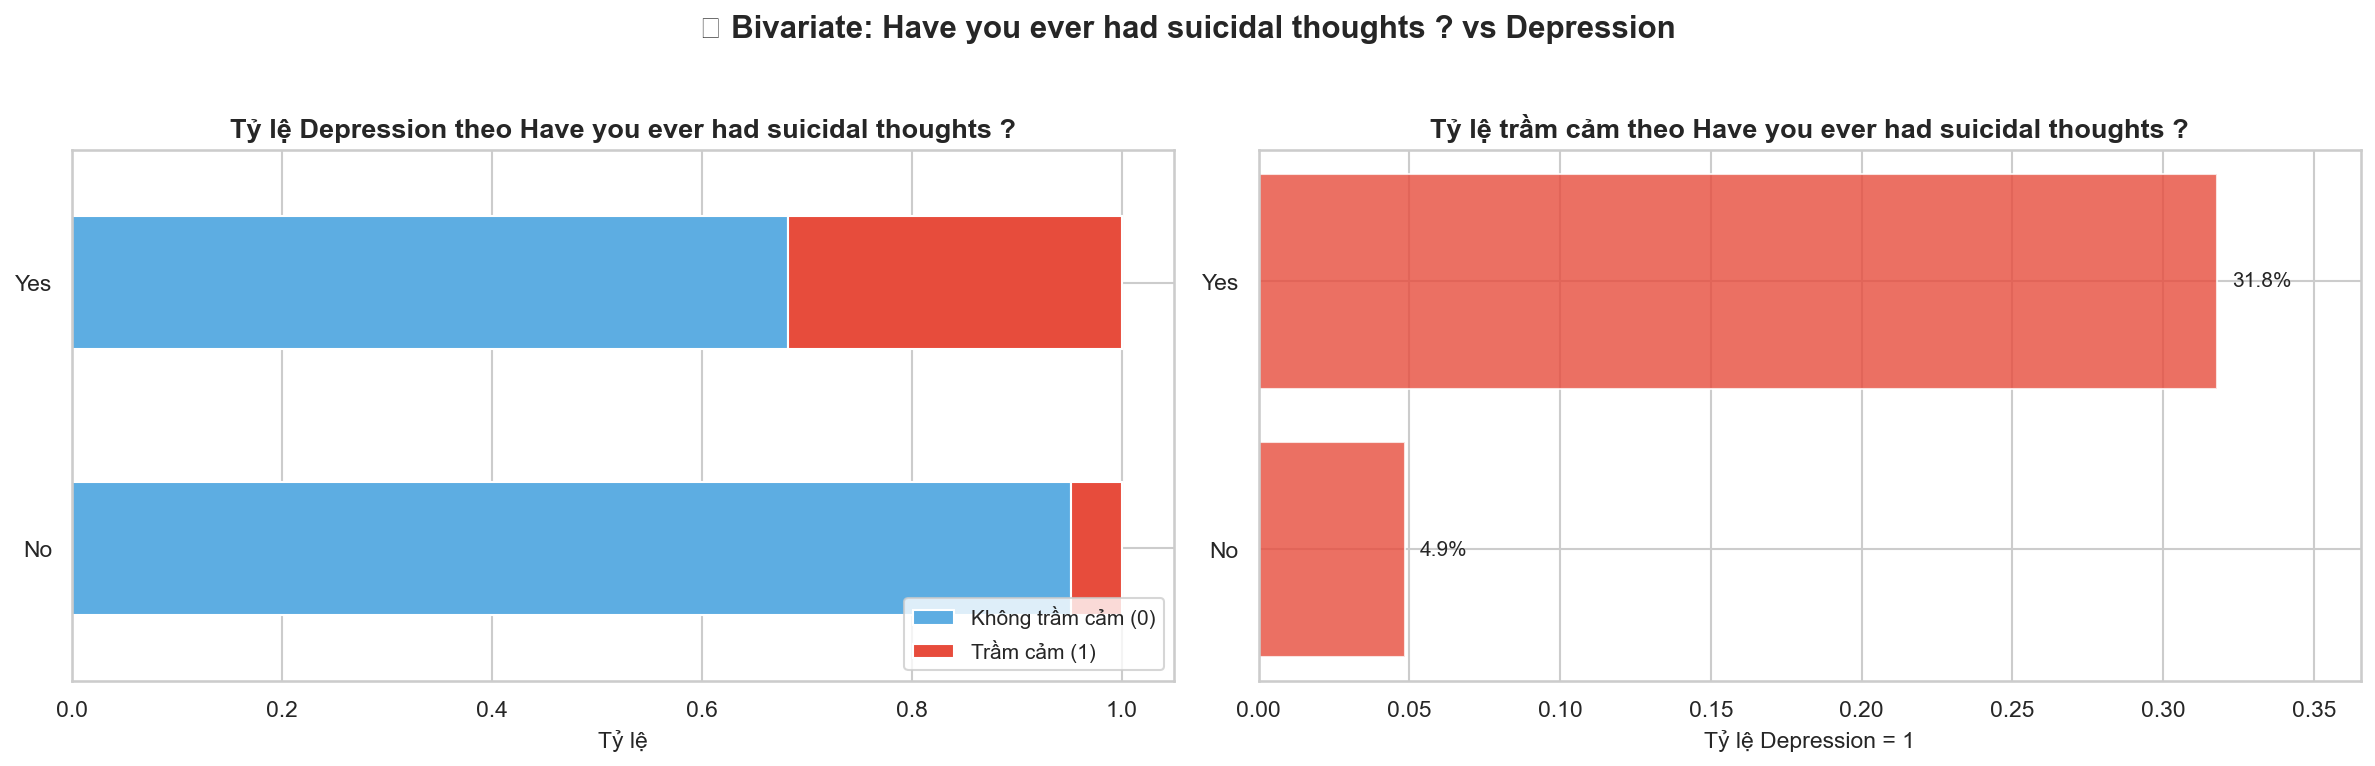
\includegraphics[width=0.95\textwidth]{eda/suicidal_vs_dep.png}
\caption{Phân tích Suicidal Thoughts vs Depression: tỷ lệ (trái) và depression rate (phải)}
\label{fig:suicidal_vs_dep}
\end{figure}

\subsection{Phân tích tương quan}
\label{subsec:correlation}

Hình~\ref{fig:corr_heatmap} trình bày ma trận tương quan Pearson giữa các đặc trưng số. Một số quan sát đáng chú ý:

\begin{itemize}[noitemsep]
    \item \textbf{Age} có tương quan âm mạnh nhất với Depression ($r = -0,565$), cho thấy người trẻ tuổi có nguy cơ trầm cảm cao hơn.
    \item \textbf{Academic Pressure} có tương quan dương mạnh ($r = 0,475$).
    \item \textbf{Job Satisfaction} và \textbf{Study Satisfaction} có $r = -1,0$ --- đây là hiện tượng multicollinearity hoàn hảo do cơ chế sinh dữ liệu (hai biến này thuộc hai nhóm đối tượng khác nhau), cần được xử lý bằng cách merge ở bước tiền xử lý.
\end{itemize}

\begin{figure}[H]
\centering
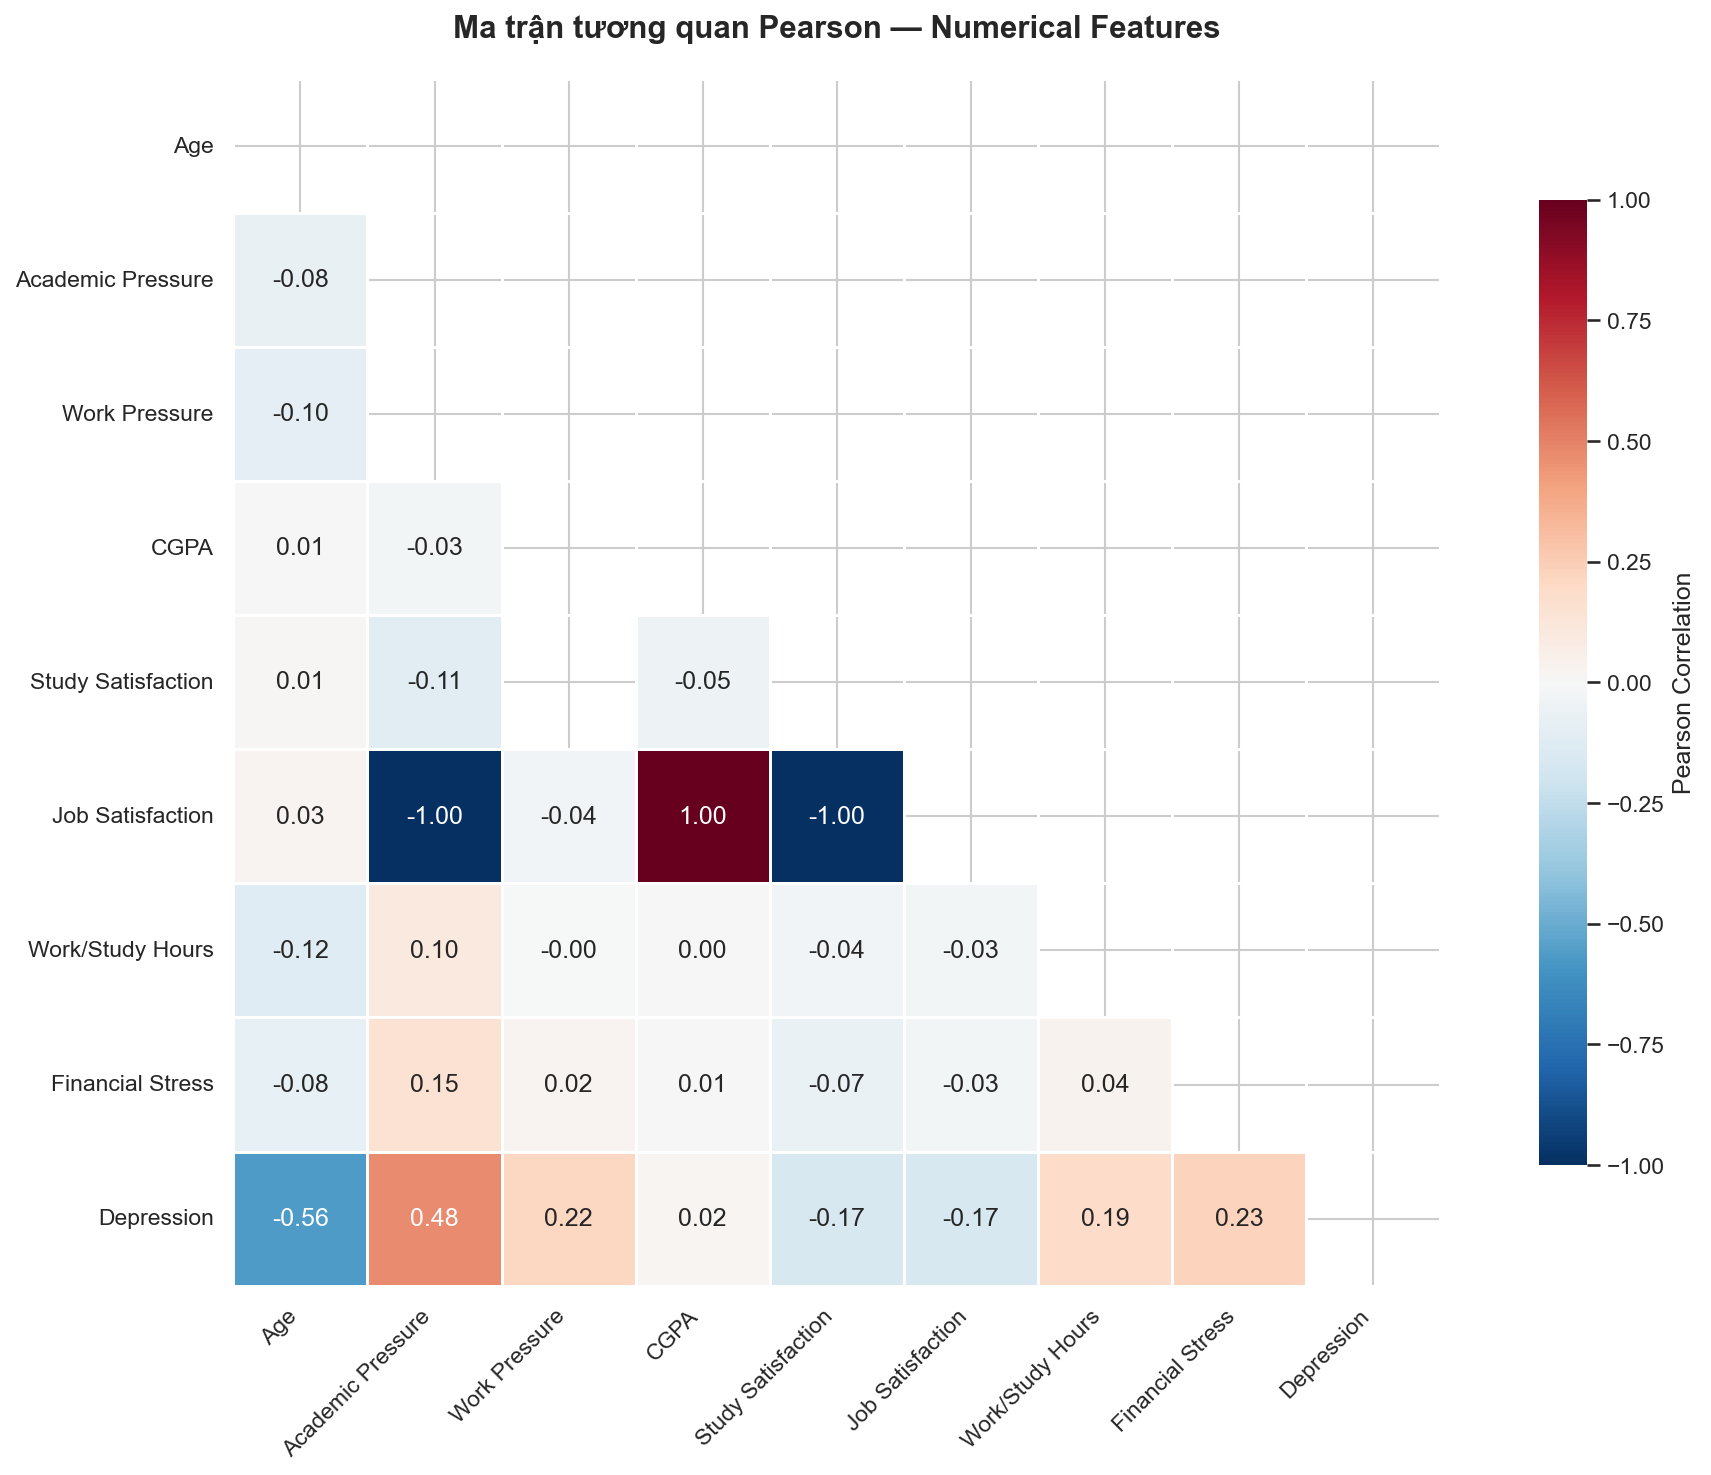
\includegraphics[width=0.75\textwidth]{eda/correlation_heatmap.png}
\caption{Ma trận tương quan Pearson giữa các đặc trưng số}
\label{fig:corr_heatmap}
\end{figure}

Hình~\ref{fig:top_corr} xếp hạng các đặc trưng theo mức tương quan tuyệt đối với Depression. Năm đặc trưng có tương quan mạnh nhất lần lượt là: Age ($-0,565$), Academic Pressure ($0,475$), Financial Stress ($0,227$), Work Pressure ($0,217$) và Work/Study Hours ($0,192$).

\begin{figure}[H]
\centering
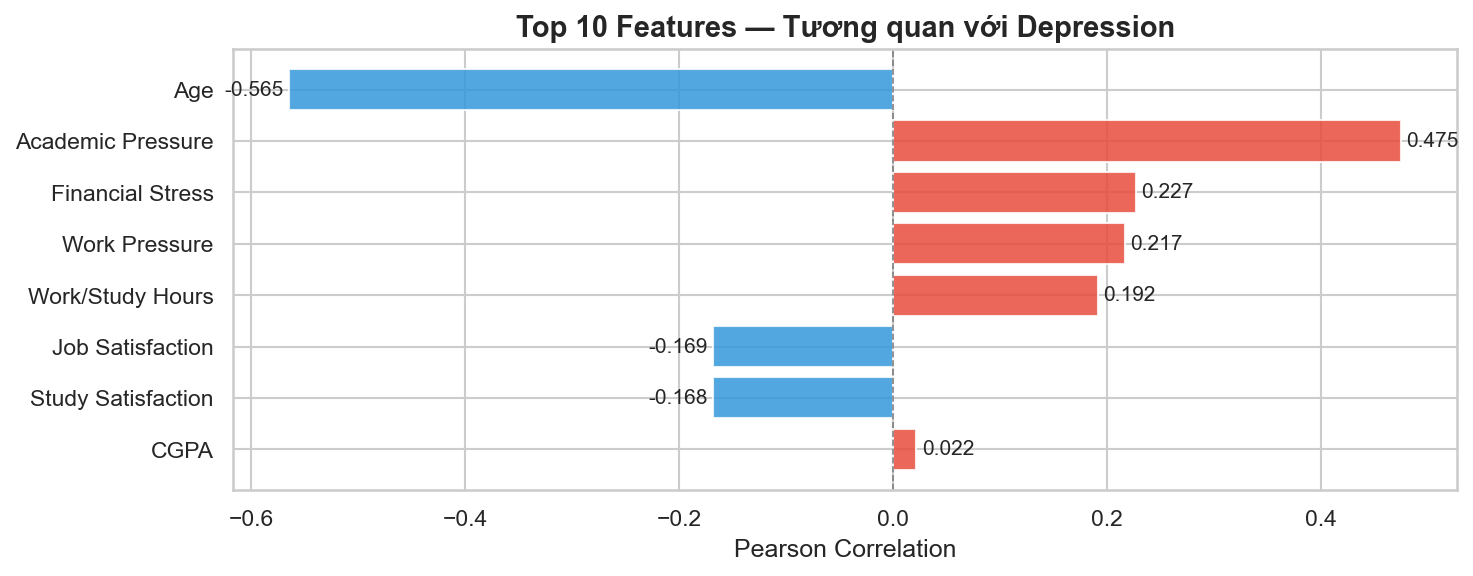
\includegraphics[width=0.85\textwidth]{eda/top_correlations.png}
\caption{Top đặc trưng có tương quan mạnh nhất với Depression}
\label{fig:top_corr}
\end{figure}

\subsection{Phân tích đa biến (Multivariate Analysis)}
\label{subsec:multivariate}

Ngoài phân tích từng đặc trưng riêng lẻ, nhóm tác giả khám phá các tương tác đa biến (\textit{interaction patterns}) để hiểu sâu hơn về cơ chế tác động lên Depression.

\textbf{Suicidal Thoughts $\times$ Family History $\rightarrow$ Depression} (Hình~\ref{fig:multi_suicidal_family}): Kết quả cho thấy hiệu ứng cộng gộp rõ ràng. Khi cả hai yếu tố cùng xuất hiện (Suicidal Thoughts = Yes, Family History = Yes), tỷ lệ trầm cảm đạt 32,6\%. Ngược lại, khi cả hai đều không có, tỷ lệ chỉ 4,7\%. Đặc biệt, yếu tố Suicidal Thoughts đóng vai trò quyết định hơn Family History: nhóm (Yes, No) có tỷ lệ 30,9\% trong khi nhóm (No, Yes) chỉ 5,0\%.

\begin{figure}[H]
\centering
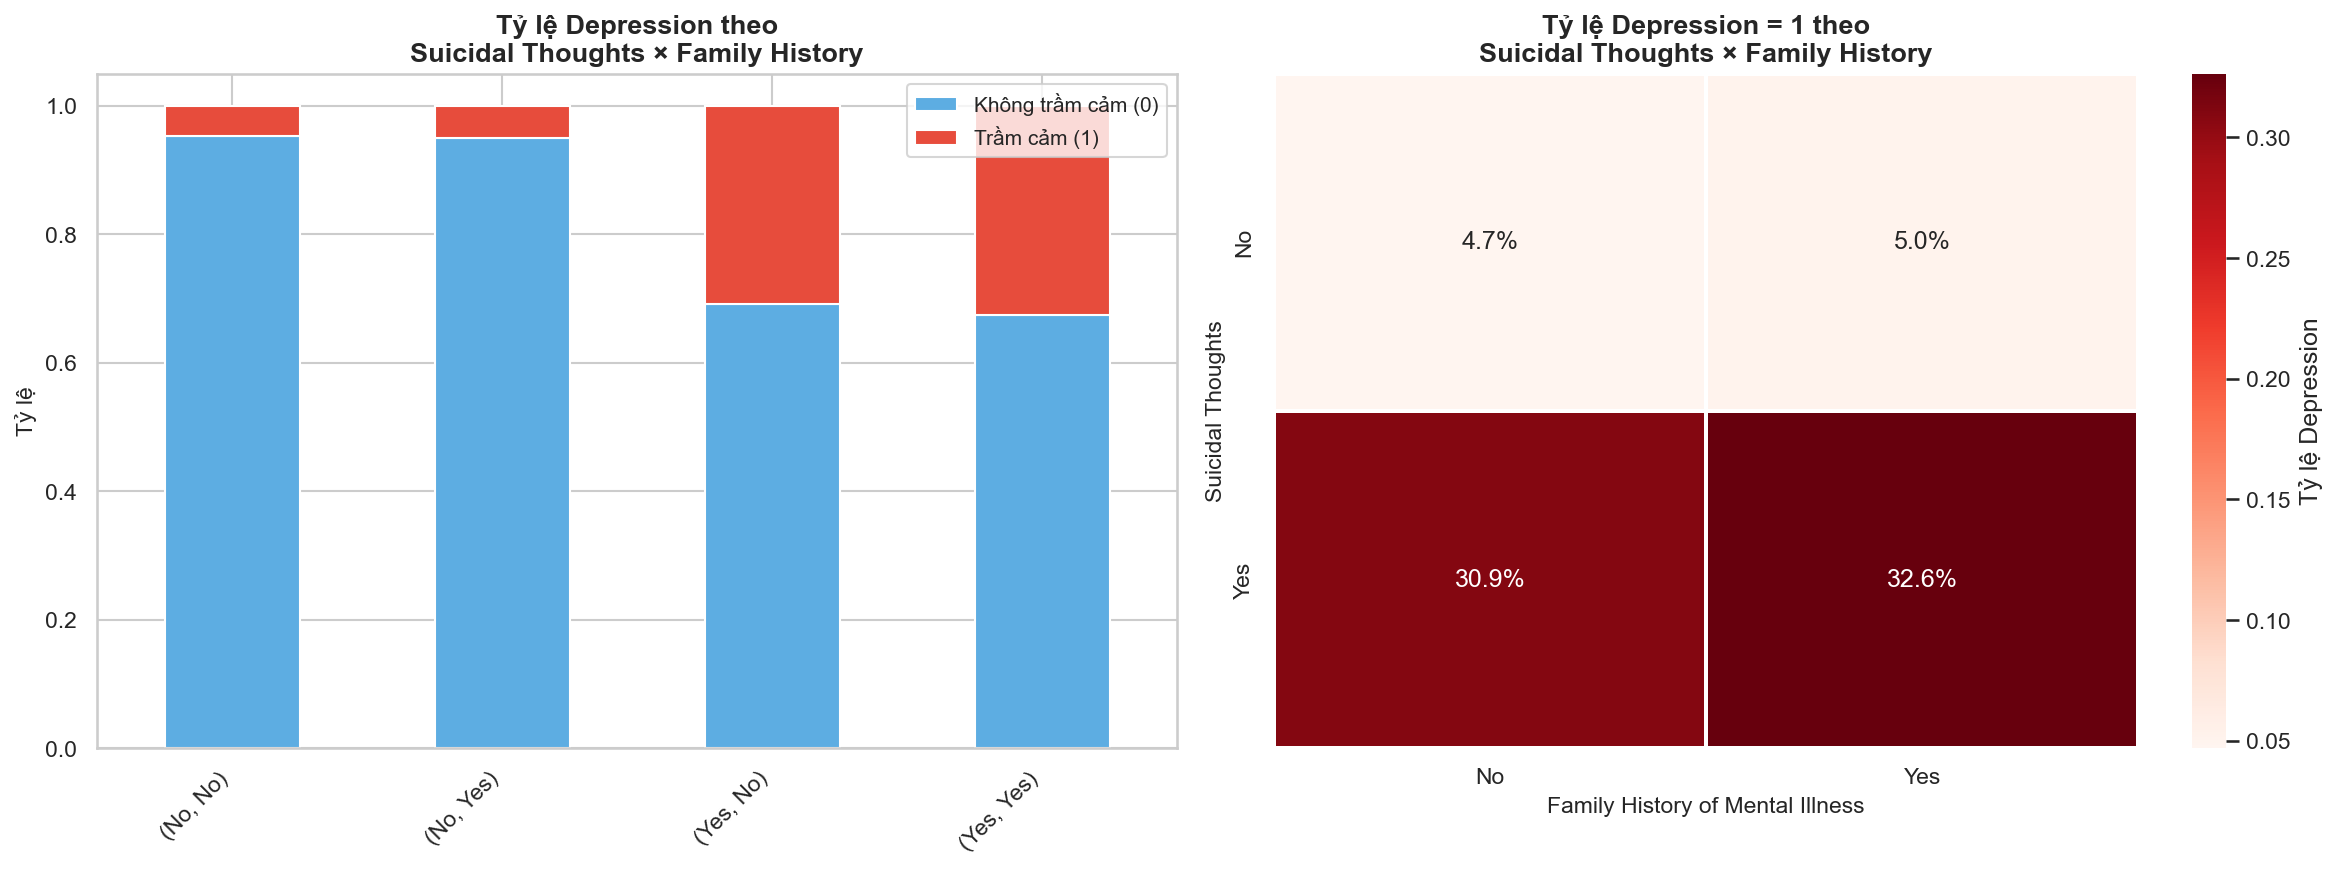
\includegraphics[width=0.95\textwidth]{eda/multivariate_suicidal_family.png}
\caption{Tương tác Suicidal Thoughts $\times$ Family History và tỷ lệ Depression}
\label{fig:multi_suicidal_family}
\end{figure}

Các interaction patterns này là \textbf{tiền đề trực tiếp} cho việc tạo các đặc trưng tương tác (\textit{interaction features}) ở Mục~\ref{sec:feature_eng}, cụ thể là đặc trưng \texttt{risk\_score} kết hợp Suicidal Thoughts và Family History.

\subsection{Các phát hiện chính}
\label{subsec:key_findings}

Từ quá trình khám phá dữ liệu, nhóm tác giả rút ra các phát hiện quan trọng sau:

\begin{enumerate}[noitemsep]
    \item \textbf{Tuổi là yếu tố dự đoán mạnh nhất}: Người trẻ (18--30 tuổi) có nguy cơ trầm cảm cao gấp nhiều lần so với nhóm trung niên và lớn tuổi.
    \item \textbf{Dữ liệu mất cân bằng vừa phải}: Tỷ lệ 81,8\% vs 18,2\% cần được cân nhắc khi đánh giá mô hình.
    \item \textbf{Áp lực học tập/công việc và căng thẳng tài chính} có tương quan dương đáng kể với trầm cảm.
    \item \textbf{Suy nghĩ tự tử} là dấu hiệu cảnh báo mạnh nhất trong các đặc trưng nhị phân.
    \item \textbf{Missing values có cấu trúc MNAR}: 5 cột chỉ tồn tại cho một nhóm đối tượng (sinh viên hoặc người đi làm), cần chiến lược xử lý đặc biệt.
    \item \textbf{Dữ liệu bẩn (noisy data)}: Cột Sleep Duration và Dietary Habits chứa các giá trị lỗi do swap dữ liệu.
    \item \textbf{Hiệu ứng tương tác đa biến}: Sự kết hợp nhiều yếu tố rủi ro làm tăng đáng kể tỷ lệ trầm cảm, gợi ý việc tạo interaction features.
\end{enumerate}

\section{Tiền xử lý dữ liệu}
\label{sec:preprocessing}

\subsection{Làm sạch dữ liệu bẩn (Noisy Data)}
\label{subsec:noisy_data}

Trong quá trình khám phá dữ liệu, nhóm phát hiện hai cột chứa dữ liệu bẩn nghiêm trọng do lỗi nhập liệu (\textit{data entry error}) hoặc hoán đổi cột (\textit{column swap}):

\begin{itemize}[noitemsep]
    \item \textbf{Sleep Duration}: Có 36 giá trị unique thay vì 4 giá trị hợp lệ. Khoảng 79 mẫu chứa các giá trị bất thường như tên thành phố (\texttt{Pune}), tên cột (\texttt{Work\_Study\_Hours}), hoặc số giờ vô nghĩa (\texttt{45-48 hours}).
    \item \textbf{Dietary Habits}: Có 23 giá trị unique thay vì 3 giá trị hợp lệ. Khoảng 27 mẫu chứa tên bằng cấp (\texttt{BSc}), giới tính (\texttt{Male}), hoặc các giá trị bị swap từ cột khác.
\end{itemize}

Chiến lược xử lý: ánh xạ (\textit{map}) các giá trị bẩn về category hợp lệ gần nhất dựa trên ngữ nghĩa; các giá trị không thể ánh xạ được thay thế bằng giá trị mode. Bảng~\ref{tab:noisy_data} tóm tắt kết quả trước và sau khi làm sạch.

\begin{table}[H]
\centering
\caption{Kết quả làm sạch dữ liệu bẩn}
\label{tab:noisy_data}
\begin{tabular}{lccl}
\toprule
\textbf{Cột} & \textbf{Unique (trước)} & \textbf{Unique (sau)} & \textbf{Ví dụ giá trị bẩn} \\
\midrule
Sleep Duration & 36 & 4 & Pune, 45-48 hours, 10-6 hours \\
Dietary Habits & 23 & 3 & BSc, Male, 1.0 \\
\bottomrule
\end{tabular}
\end{table}

\subsection{Xử lý Missing Values}
\label{subsec:missing_values}

Hình~\ref{fig:missing_values} trình bày tỷ lệ missing values theo từng cột. Ba cột có tỷ lệ missing cao nhất là Study Satisfaction, Academic Pressure và CGPA (đều 80,17\%), tiếp theo là Profession (26,03\%), Job Satisfaction và Work Pressure (đều 19,84\%).

\begin{figure}[H]
\centering
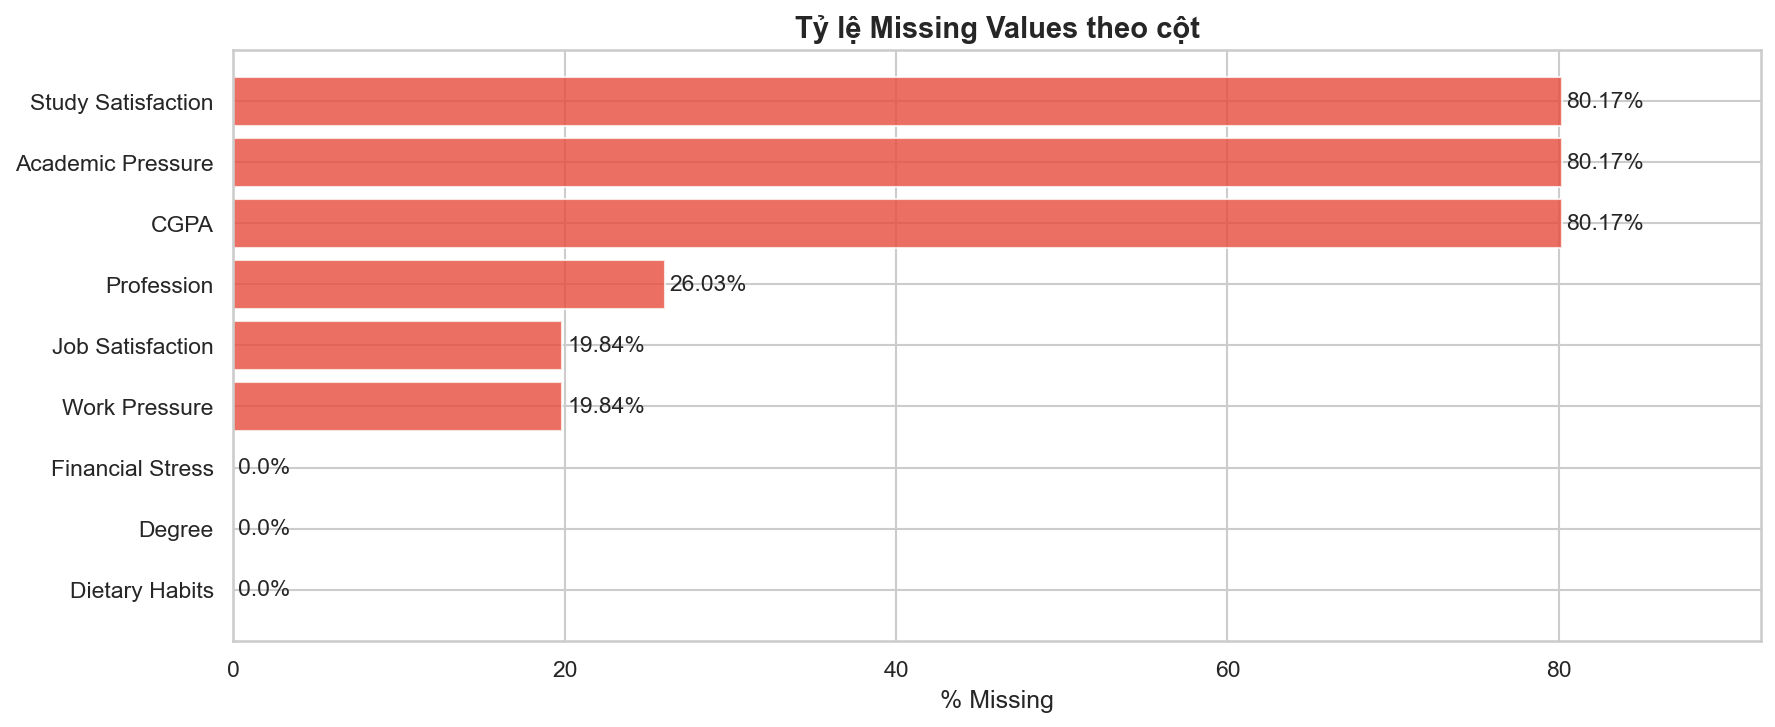
\includegraphics[width=0.85\textwidth]{preprocessing/missing_values.png}
\caption{Tỷ lệ Missing Values theo từng cột}
\label{fig:missing_values}
\end{figure}

Điểm quan trọng là các giá trị missing này \textbf{không phải ngẫu nhiên} mà thuộc loại \textbf{MNAR} (\textit{Missing Not At Random}). Hình~\ref{fig:missing_pattern} chứng minh rõ: Academic Pressure, CGPA, Study Satisfaction chỉ có giá trị ở nhóm Student (100\% missing ở Working Professional), trong khi Work Pressure và Job Satisfaction chỉ có ở Working Professional (100\% missing ở Student). Đây là thiết kế có chủ đích của bộ dữ liệu, không phải lỗi thu thập.

\begin{figure}[H]
\centering
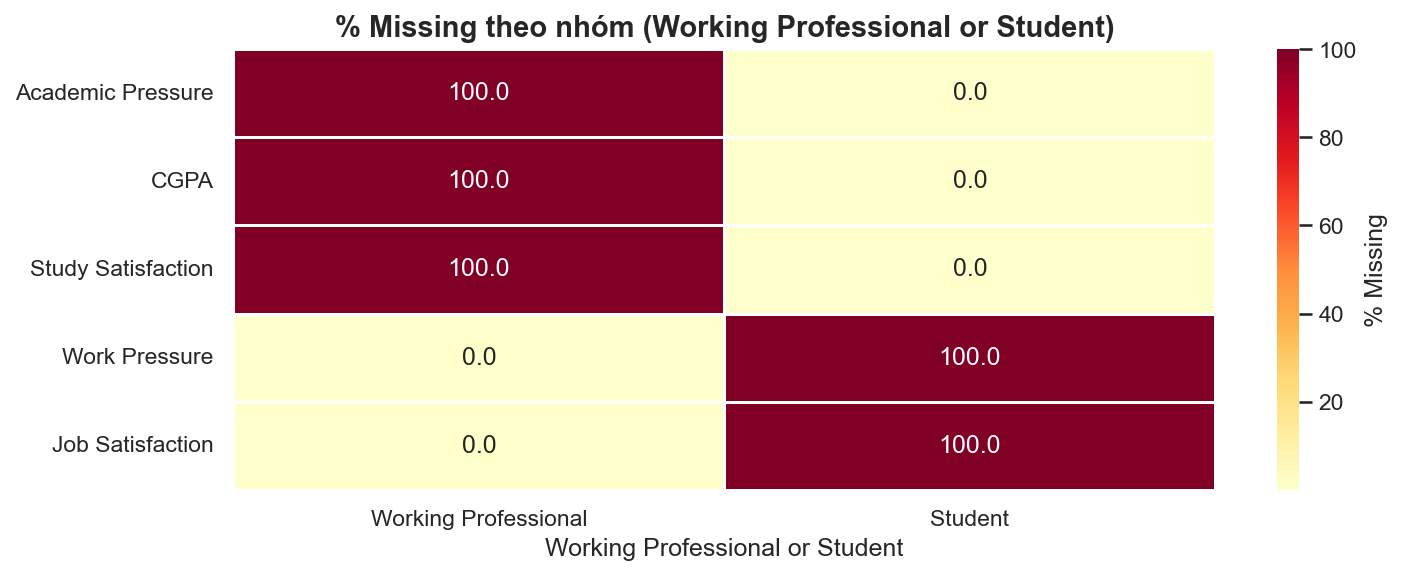
\includegraphics[width=0.85\textwidth]{preprocessing/missing_pattern_by_group.png}
\caption{Pattern Missing Values theo nhóm Working Professional vs Student}
\label{fig:missing_pattern}
\end{figure}

\subsection{Gộp các cột điều kiện (Merge Conditional Columns)}
\label{subsec:merge_columns}

Do cơ chế MNAR được phát hiện ở Mục~\ref{subsec:missing_values}, việc điền missing bằng mean/median là \textbf{không phù hợp} --- vì giá trị missing mang ý nghĩa thực sự (sinh viên không có Work Pressure, người đi làm không có Academic Pressure). Nhóm áp dụng chiến lược gộp cột (\textit{merge}) như sau:

\begin{itemize}[noitemsep]
    \item \texttt{Academic Pressure} + \texttt{Work Pressure} $\rightarrow$ \texttt{Pressure}: gộp thành một biến thống nhất đo mức áp lực chung.
    \item \texttt{Study Satisfaction} + \texttt{Job Satisfaction} $\rightarrow$ \texttt{Satisfaction}: gộp thành biến đo mức hài lòng chung.
    \item \texttt{CGPA}: giữ nguyên, đồng thời tạo thêm biến nhị phân \texttt{has\_cgpa} để đánh dấu đối tượng là sinh viên hay không.
\end{itemize}

Kết quả: số lượng đặc trưng giảm từ 20 xuống 17, đồng thời loại bỏ hoàn toàn vấn đề missing values cho 5 cột điều kiện.

\subsection{Loại bỏ đặc trưng không cần thiết}
\label{subsec:drop_features}

Cột \texttt{Name} được loại bỏ vì chứa thông tin định danh cá nhân, không có giá trị dự đoán cho biến mục tiêu Depression.

\subsection{Mã hóa biến phân loại (Encoding Categorical Variables)}
\label{subsec:encoding}

Các biến phân loại được mã hóa theo hai phương pháp phù hợp:

\begin{itemize}[noitemsep]
    \item \textbf{Binary Encoding}: Áp dụng cho các biến nhị phân --- \texttt{Gender} (Male=1, Female=0), \texttt{Suicidal Thoughts} (Yes=1, No=0), \texttt{Family History} (Yes=1, No=0), \texttt{Working Professional or Student} (Student=0, Professional=1).
    \item \textbf{Ordinal Encoding}: Áp dụng cho các biến có thứ tự tự nhiên --- \texttt{Sleep Duration} (Less than 5h=0, 5-6h=1, 7-8h=2, More than 8h=3) và \texttt{Dietary Habits} (Unhealthy=0, Moderate=1, Healthy=2).
\end{itemize}

Lý do không sử dụng One-Hot Encoding: các biến này có thứ tự rõ ràng (ít $\rightarrow$ nhiều, xấu $\rightarrow$ tốt), ordinal encoding bảo toàn thông tin thứ tự này.

\subsection{Chuẩn hóa đặc trưng (Feature Scaling)}
\label{subsec:scaling}

Chuẩn hóa đặc trưng chỉ cần thiết cho các mô hình nhạy cảm với thang đo như Logistic Regression và SVM. Các mô hình tree-based (Decision Tree, Random Forest, XGBoost, LightGBM) không yêu cầu chuẩn hóa.

\textbf{Standardization} (Z-score normalization) --- dịch chuyển và co giãn dữ liệu sao cho trung bình bằng 0 và độ lệch chuẩn bằng 1. Lưu ý rằng phương pháp này \textbf{không} biến đổi hình dạng phân phối gốc về phân phối chuẩn (Gaussian), mà chỉ chuẩn hóa thang đo:

\begin{equation}
z = \frac{x - \mu}{\sigma}
\label{eq:standardization}
\end{equation}

trong đó $x$ là giá trị gốc, $\mu$ là trung bình mẫu và $\sigma$ là độ lệch chuẩn mẫu của đặc trưng.

\textbf{Min-Max Normalization} --- co giãn giá trị về khoảng $[0, 1]$:

\begin{equation}
x' = \frac{x - x_{\min}}{x_{\max} - x_{\min}}
\label{eq:minmax}
\end{equation}

trong đó $x_{\min}$ và $x_{\max}$ lần lượt là giá trị nhỏ nhất và lớn nhất của đặc trưng trong tập huấn luyện.

Trong dự án này, nhóm sử dụng \textbf{Standardization} (Phương trình~\ref{eq:standardization}) cho Logistic Regression và SVM vì phương pháp này ít bị ảnh hưởng bởi outliers hơn Min-Max.

\subsection{Kết quả tiền xử lý}
\label{subsec:preprocessing_result}

Bảng~\ref{tab:preprocessing_result} tóm tắt kết quả trước và sau quá trình tiền xử lý dữ liệu.

\begin{table}[H]
\centering
\caption{So sánh dữ liệu trước và sau tiền xử lý}
\label{tab:preprocessing_result}
\begin{tabular}{lcc}
\toprule
\textbf{Tiêu chí} & \textbf{Trước} & \textbf{Sau} \\
\midrule
Số đặc trưng & 20 & 17 \\
Số dòng (train) & 140.700 & 140.700 \\
Missing values & Có (5 cột, lên tới 80\%) & 0 \\
Noisy data & Có (2 cột) & 0 \\
Kiểu dữ liệu & Hỗn hợp (text + số) & Hoàn toàn số \\
\bottomrule
\end{tabular}
\end{table}

\section{Kỹ thuật đặc trưng (Feature Engineering)}
\label{sec:feature_eng}

\subsection{Mã hóa đặc trưng High Cardinality --- Target Encoding}
\label{subsec:target_encoding}

Ba đặc trưng phân loại \texttt{City}, \texttt{Profession} và \texttt{Degree} có số lượng category rất lớn (hàng chục đến hàng trăm giá trị unique), khiến One-Hot Encoding không khả thi vì sẽ tạo quá nhiều cột thưa. Nhóm tác giả áp dụng \textbf{Target Encoding} --- thay thế mỗi category bằng giá trị trung bình của biến mục tiêu trong category đó, kết hợp smoothing để giảm overfitting:

\begin{equation}
\text{TargetEnc}(c) = \frac{\displaystyle\sum_{i:\, x_i = c} y_i + \lambda \cdot \bar{y}}{n_c + \lambda}
\label{eq:target_encoding}
\end{equation}

trong đó:
\begin{itemize}[noitemsep]
    \item $c$: category cần mã hóa
    \item $n_c$: số lần category $c$ xuất hiện trong tập dữ liệu
    \item $\bar{y}$: giá trị trung bình của biến mục tiêu trên toàn bộ tập dữ liệu (global mean)
    \item $\lambda$: hệ số smoothing, kiểm soát mức độ ``co về'' global mean
\end{itemize}

Khi $n_c$ nhỏ (category hiếm), giá trị encoding bị kéo về $\bar{y}$ nhiều hơn, giúp tránh overfitting. Để ngăn ngừa data leakage, Target Encoding được thực hiện trong vòng lặp Cross-Validation: chỉ fit trên tập train của mỗi fold và transform trên tập validation.

\subsection{Phân nhóm tuổi (Age Binning)}
\label{subsec:age_binning}

Dựa trên phân tích EDA (Mục~\ref{subsec:bivariate}), nhóm tác giả nhận thấy mối quan hệ giữa tuổi và trầm cảm không tuyến tính đơn thuần mà có sự khác biệt rõ rệt theo nhóm tuổi. Do đó, kỹ thuật \textit{Discretization/Binning} được áp dụng để chia \texttt{Age} thành 4 nhóm ordinal:

\begin{itemize}[noitemsep]
    \item Nhóm 0: 18--29 tuổi (tỷ lệ trầm cảm 57,0\%)
    \item Nhóm 1: 30--42 tuổi (tỷ lệ trầm cảm 12,8\%)
    \item Nhóm 2: 43--51 tuổi (tỷ lệ trầm cảm 1,7\%)
    \item Nhóm 3: 52+ tuổi (tỷ lệ trầm cảm 0,3\%)
\end{itemize}

Hình~\ref{fig:age_group} minh họa sự khác biệt rất lớn về tỷ lệ trầm cảm giữa các nhóm tuổi: nhóm 18--29 có tỷ lệ gấp gần 200 lần so với nhóm 52+, đồng thời số lượng mẫu phân bố tương đối đồng đều giữa 4 nhóm (~32.000--38.000 mẫu/nhóm).

\begin{figure}[H]
\centering

\includegraphics[width=0.95\textwidth]{feature_eng/age_group_vs_depression.png}
\caption{Tỷ lệ Depression và số lượng mẫu theo nhóm tuổi (Age Binning)}
\label{fig:age_group}
\end{figure}

\subsection{Tạo đặc trưng tương tác (Interaction Features)}
\label{subsec:interaction_features}

Dựa trên kết quả phân tích đa biến ở Mục~\ref{subsec:multivariate}, nhóm tác giả tạo thêm các đặc trưng kết hợp nhằm nắm bắt hiệu ứng tương tác giữa nhiều yếu tố:

\textbf{Stress Load} --- đo mức tải stress tổng hợp từ áp lực và căng thẳng tài chính:
\begin{equation}
\text{stress\_load} = \text{Pressure} \times \text{Financial\_Stress}
\label{eq:stress_load}
\end{equation}

\textbf{Wellbeing Index} --- chỉ số sức khỏe tổng thể dựa trên mức hài lòng và giấc ngủ:
\begin{equation}
\text{wellbeing\_index} = \frac{\text{Satisfaction} + \text{Sleep\_Duration}}{2}
\label{eq:wellbeing}
\end{equation}

\textbf{Stress-Satisfaction Ratio} --- tỷ lệ giữa áp lực và mức hài lòng:
\begin{equation}
\text{stress\_satisfaction\_ratio} = \frac{\text{Pressure}}{\text{Satisfaction} + 1}
\label{eq:stress_ratio}
\end{equation}

\textbf{Risk Score} --- chỉ số rủi ro cộng gộp từ hai yếu tố cảnh báo mạnh nhất:
\begin{equation}
\text{risk\_score} = \text{Suicidal\_Thoughts} + \text{Family\_History}
\label{eq:risk_score}
\end{equation}

Hình~\ref{fig:interaction_cont} minh họa phân phối các đặc trưng tương tác liên tục và mối quan hệ với Depression. Nhóm trầm cảm có giá trị \texttt{stress\_load} và \texttt{stress\_satisfaction\_ratio} cao hơn rõ rệt, trong khi \texttt{wellbeing\_index} thấp hơn --- phù hợp với kỳ vọng.

\begin{figure}[H]
\centering
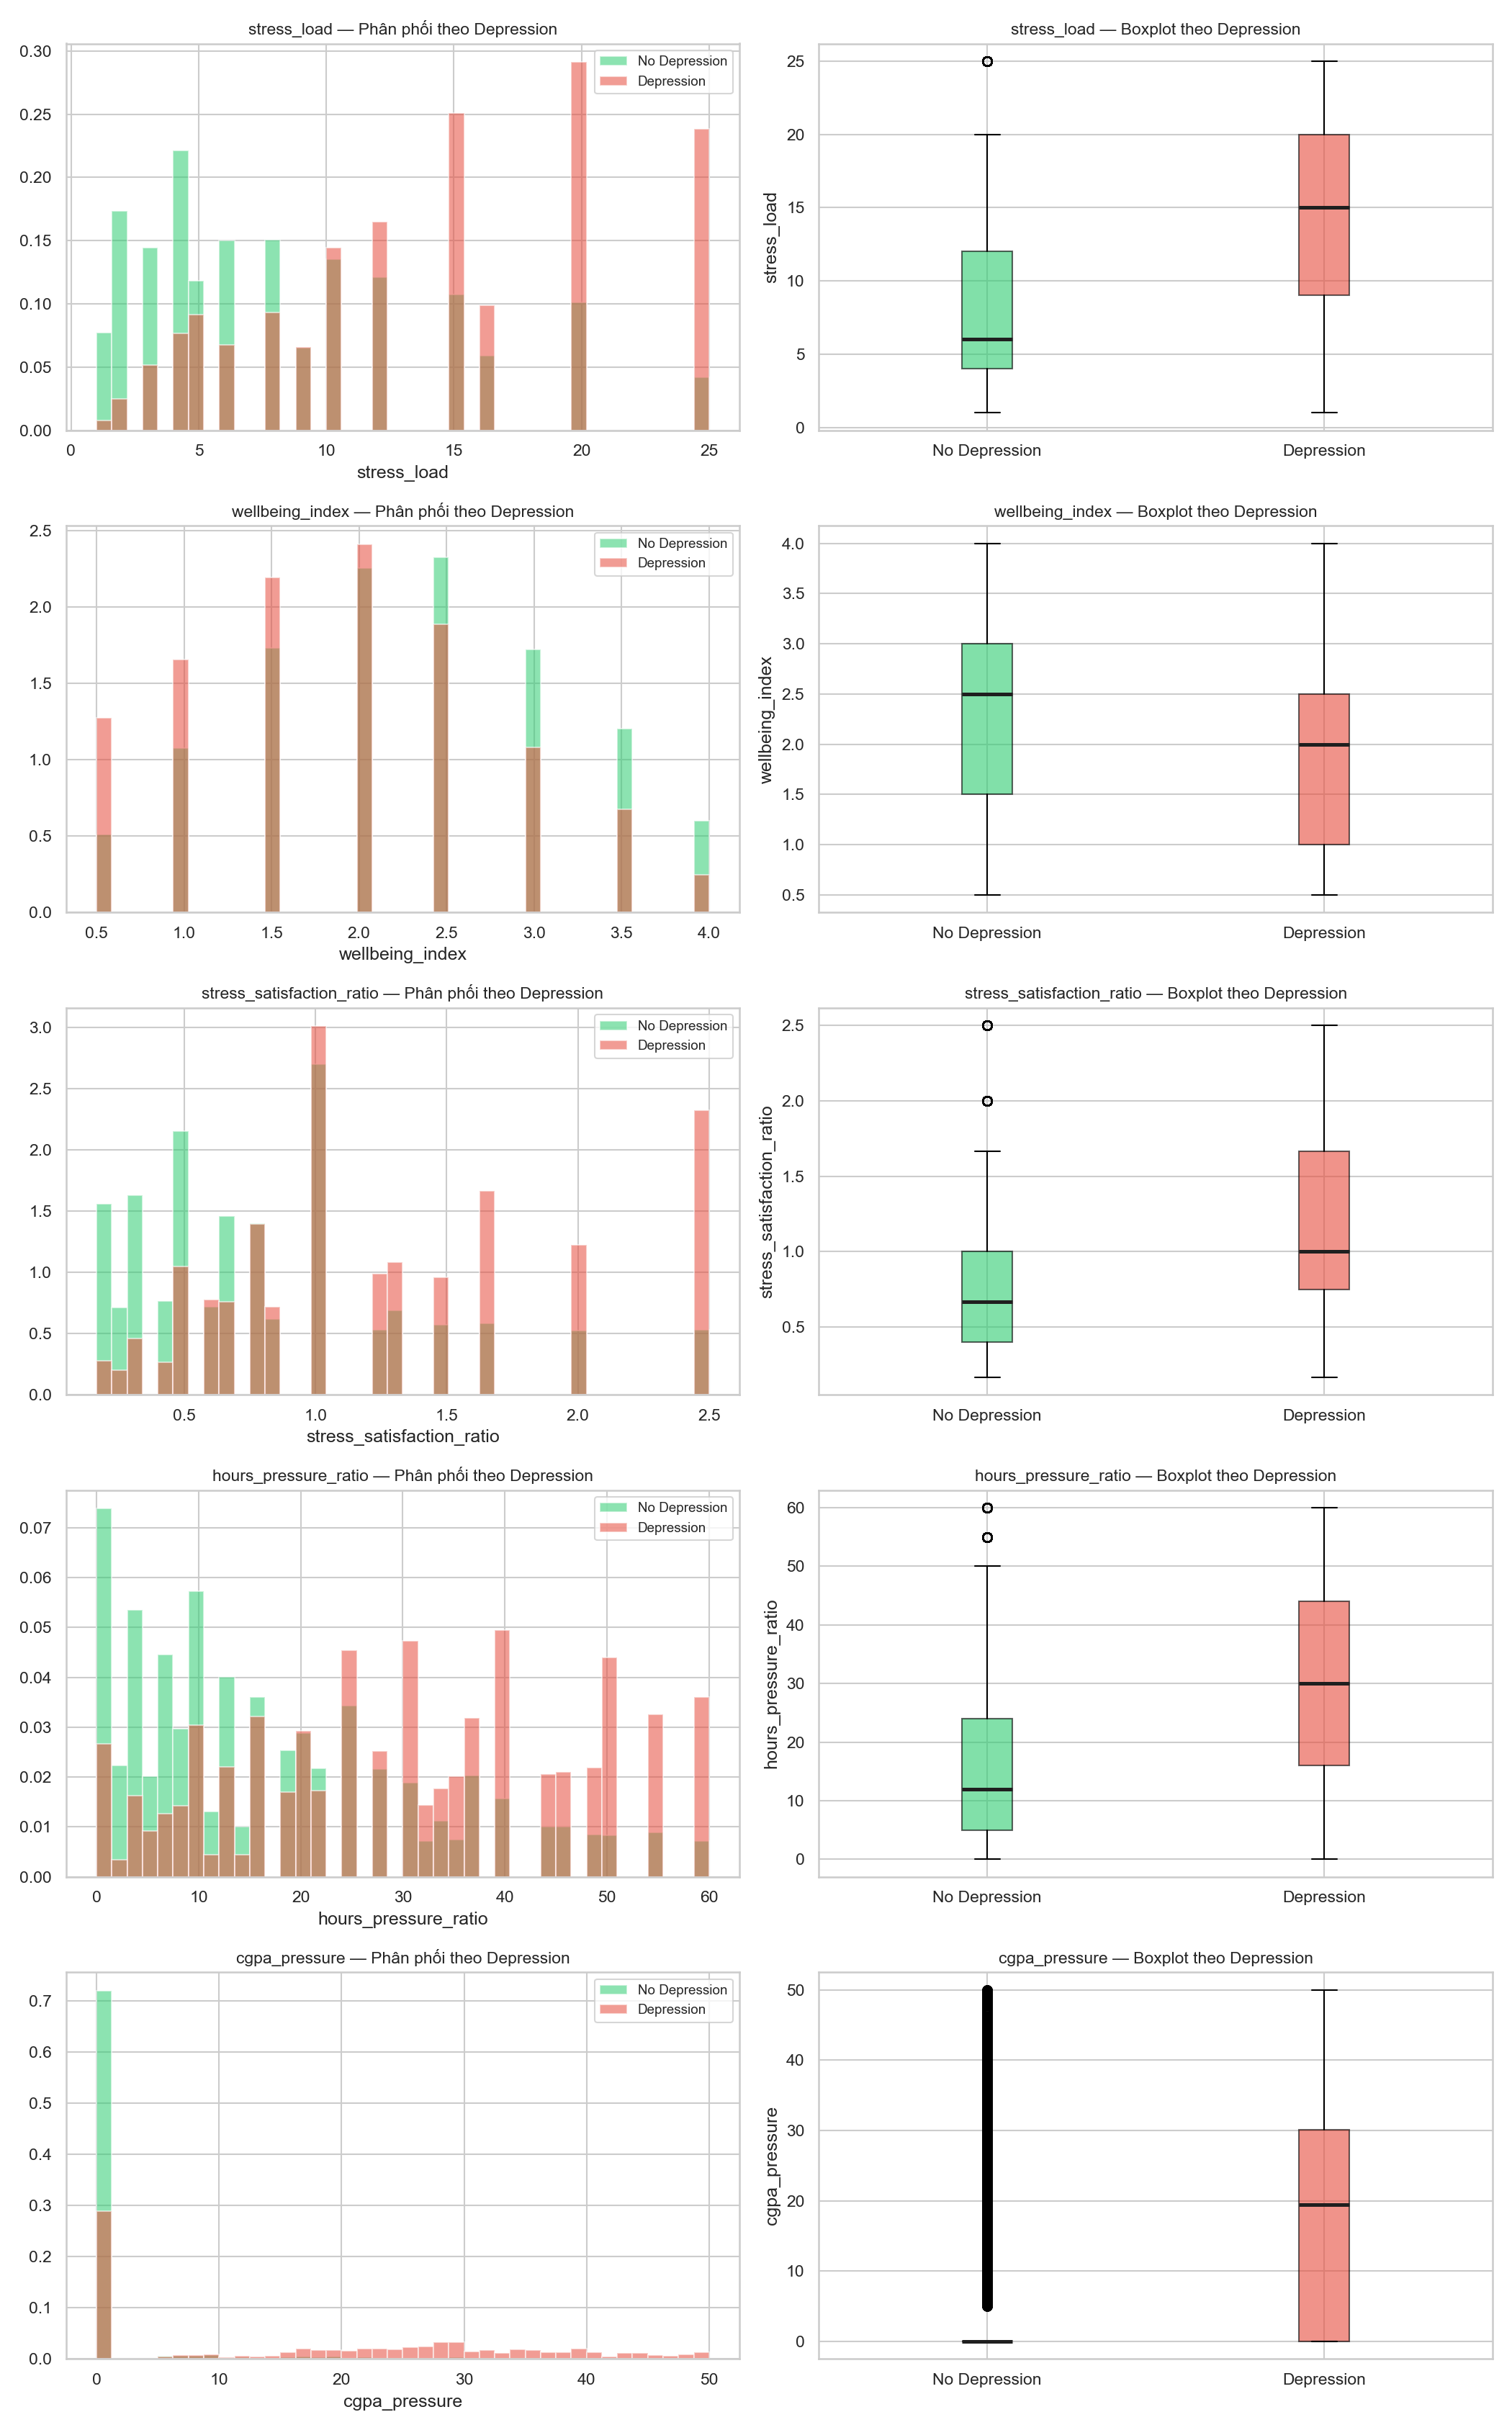
\includegraphics[width=0.95\textwidth]{feature_eng/interaction_continuous_vs_depression.png}
\caption{Phân phối và boxplot các đặc trưng tương tác liên tục theo Depression}
\label{fig:interaction_cont}
\end{figure}

Hình~\ref{fig:interaction_disc} cho thấy đặc trưng \texttt{risk\_score} có khả năng phân biệt tốt: khi score = 0, tỷ lệ trầm cảm chỉ 4,7\%; khi score = 1 là 17,9\%; và khi score = 2 (cả hai yếu tố rủi ro đều có) là 32,6\%.

\begin{figure}[H]
\centering
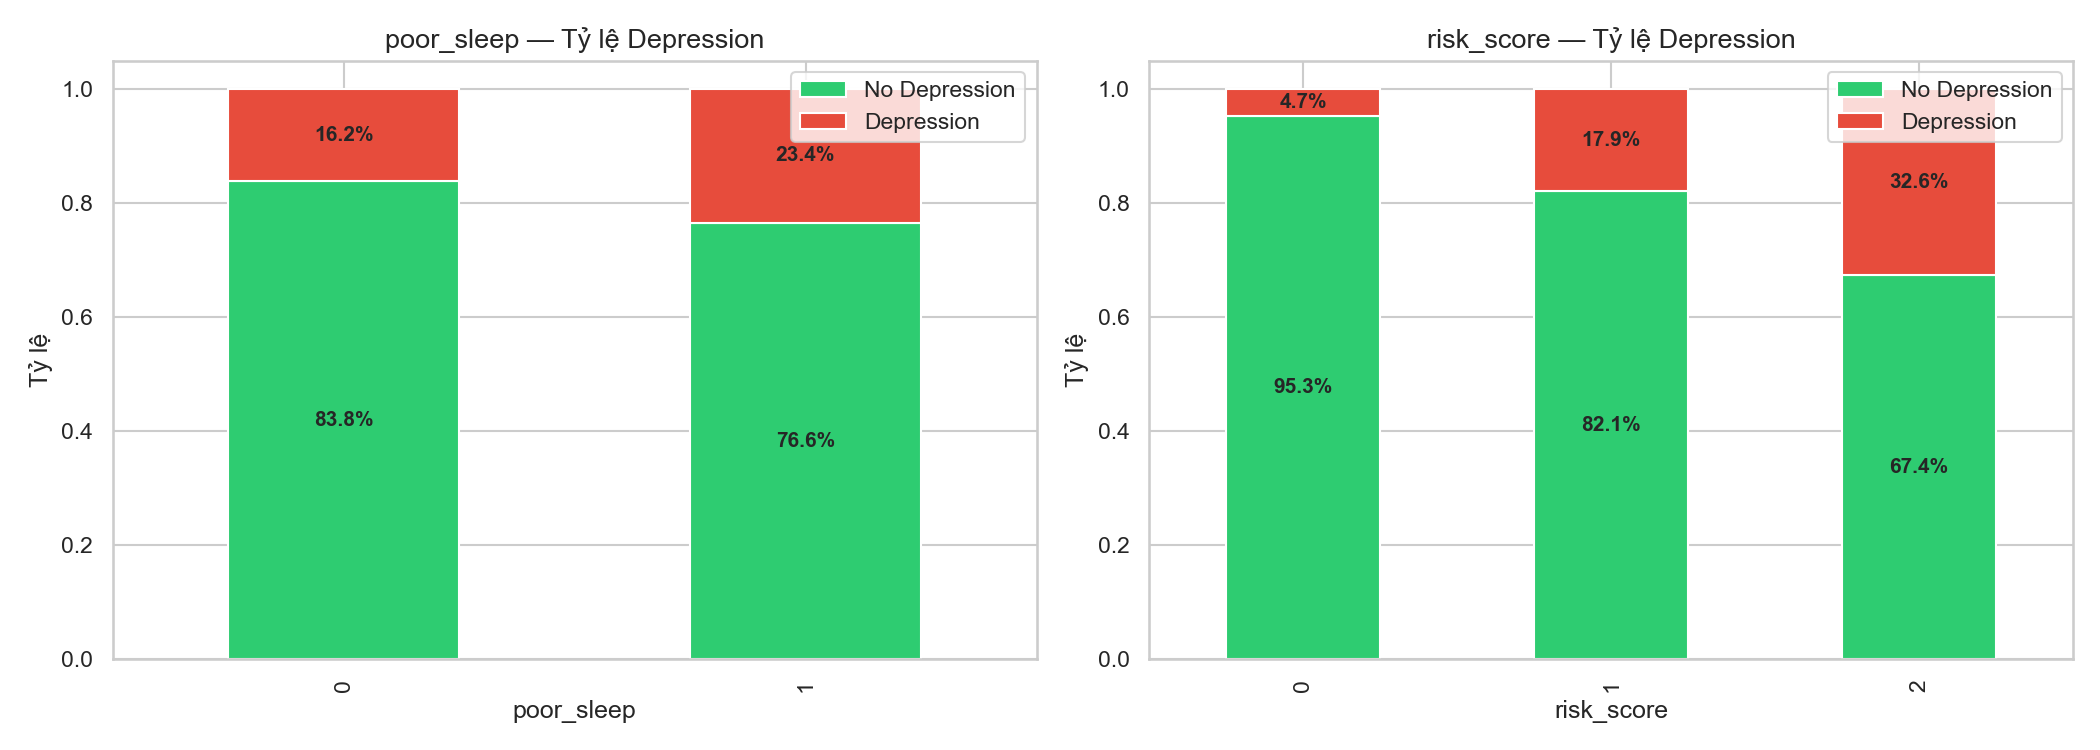
\includegraphics[width=0.95\textwidth]{feature_eng/interaction_discrete_vs_depression.png}
\caption{Tỷ lệ Depression theo poor\_sleep và risk\_score}
\label{fig:interaction_disc}
\end{figure}

\subsection{Lựa chọn đặc trưng (Feature Selection)}
\label{subsec:feature_selection}

Để đánh giá tầm quan trọng của các đặc trưng (bao gồm cả đặc trưng gốc và đặc trưng mới tạo), nhóm tác giả sử dụng \textbf{Random Forest Feature Importance} --- đo mức giảm Gini Impurity trung bình khi split trên mỗi đặc trưng.

Hình~\ref{fig:feat_importance_rf} cho thấy kết quả xếp hạng: \texttt{Age} (0,17) và \texttt{age\_group} (0,13) là hai đặc trưng quan trọng nhất, tiếp theo là \texttt{Suicidal Thoughts} (0,11), \texttt{cgpa\_pressure} (0,10) và \texttt{Profession\_te} (0,07). Đáng chú ý, các đặc trưng tương tác mới tạo (\texttt{stress\_load}, \texttt{cgpa\_pressure}, \texttt{stress\_satisfaction\_ratio}) đều nằm trong top 10, xác nhận giá trị của bước Feature Engineering.

\begin{figure}[H]
\centering
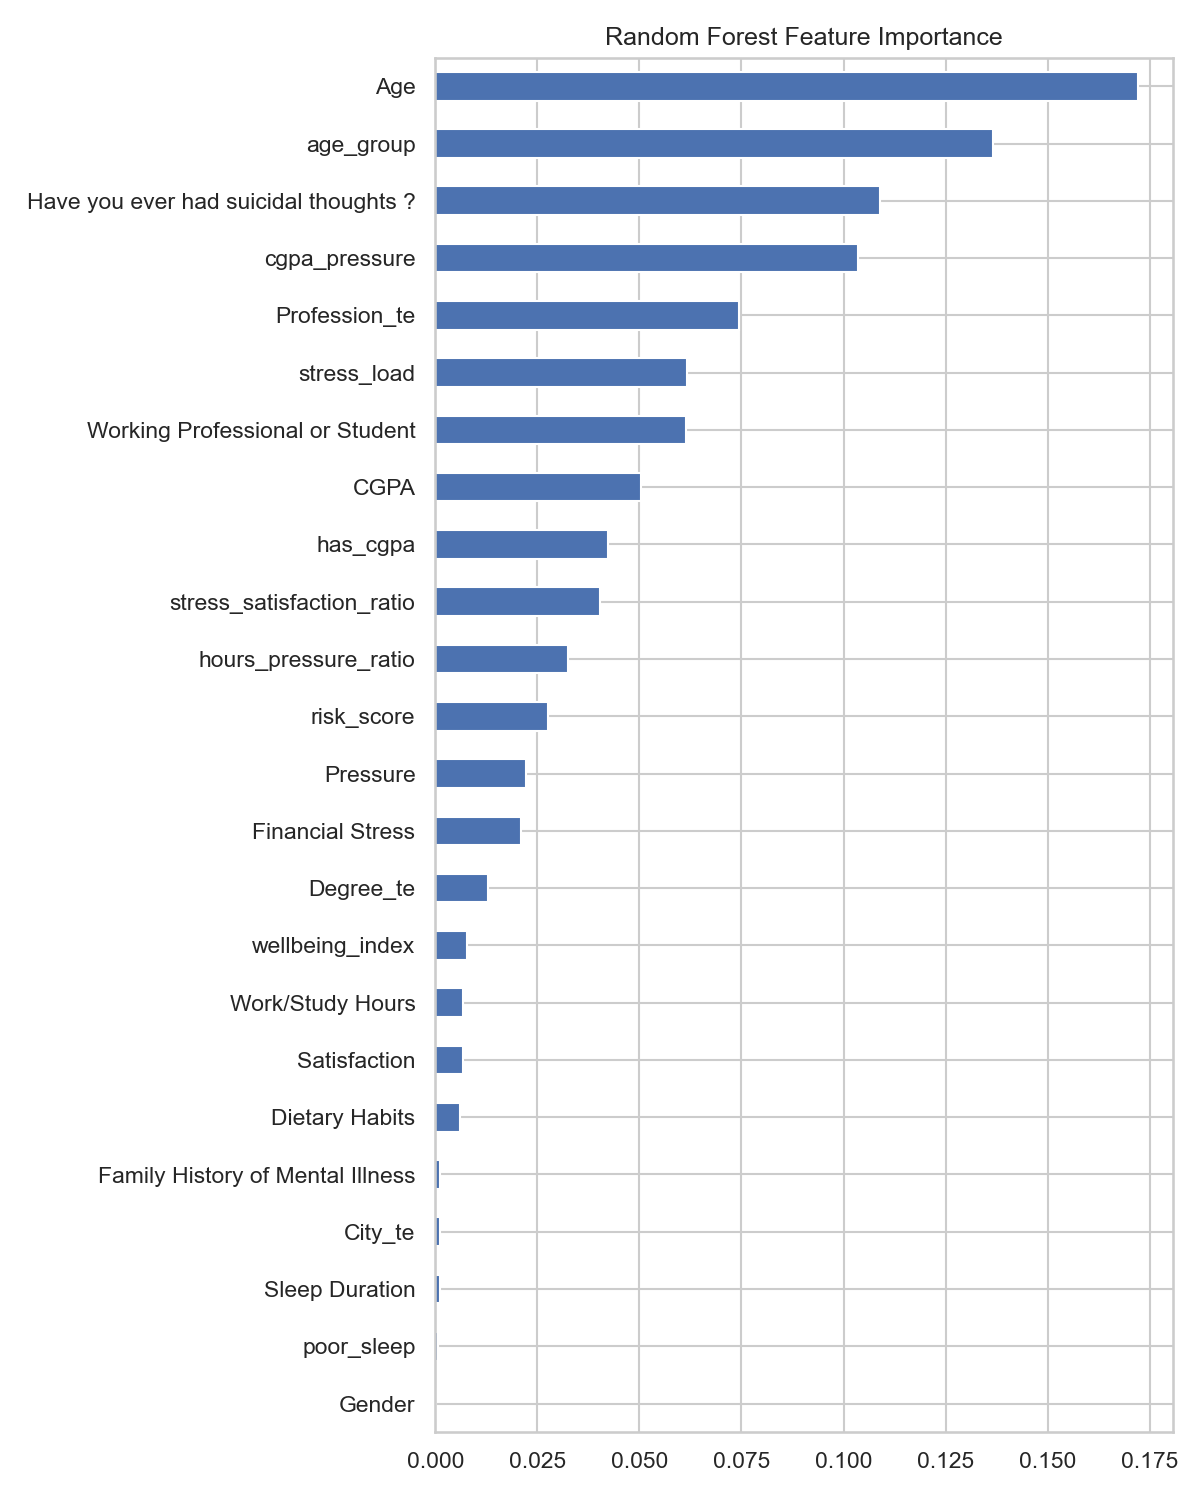
\includegraphics[width=0.7\textwidth]{feature_eng/feat_importance.png}
\caption{Random Forest Feature Importance --- xếp hạng toàn bộ đặc trưng}
\label{fig:feat_importance_rf}
\end{figure}

Kết luận: nhóm tác giả giữ lại toàn bộ đặc trưng có importance $> 0$ (tổng cộng 25 đặc trưng) để đưa vào huấn luyện mô hình, vì các mô hình tree-based có khả năng tự chọn đặc trưng quan trọng trong quá trình học.

\section{Phát triển mô hình}
\label{sec:model_dev}

\subsection{Cài đặt thực nghiệm chung}
\label{subsec:experiment_setup}

\textbf{Chiến lược đánh giá}: Toàn bộ các mô hình được đánh giá bằng \textbf{5-Fold Stratified Cross-Validation}. Phương pháp Stratified đảm bảo tỷ lệ lớp Depression (0/1) được giữ nguyên trong mỗi fold, rất quan trọng khi dữ liệu mất cân bằng (81,8\% vs 18,2\%).

\textbf{Thư viện}: scikit-learn (v1.3+), xgboost (v2.0+), lightgbm (v4.0+).

\textbf{Chiến lược tuning}: Nhóm sử dụng phương pháp \textbf{Manual Hyperparameter Tuning} --- tức là chọn và điều chỉnh siêu tham số dựa trên hiểu biết về đặc tính mô hình và quan sát thực nghiệm, thay vì sử dụng các kỹ thuật tìm kiếm tự động (Grid Search, Random Search, Bayesian Optimization). Lý do: phương pháp thủ công giúp nhóm hiểu sâu hơn về ảnh hưởng của từng siêu tham số lên hiệu suất mô hình, đồng thời phù hợp hơn với mục tiêu học thuật của đồ án.

\textbf{Các chỉ số đánh giá} được sử dụng bao gồm:

\begin{equation}
\text{Accuracy} = \frac{TP + TN}{TP + TN + FP + FN}
\label{eq:accuracy}
\end{equation}

\begin{equation}
\text{Precision} = \frac{TP}{TP + FP}, \qquad \text{Recall} = \frac{TP}{TP + FN}
\label{eq:prec_recall}
\end{equation}

\begin{equation}
F_1 = 2 \cdot \frac{\text{Precision} \cdot \text{Recall}}{\text{Precision} + \text{Recall}}
\label{eq:f1}
\end{equation}

trong đó $TP$ (True Positive) là số mẫu trầm cảm được dự đoán đúng, $TN$ (True Negative) là số mẫu không trầm cảm được dự đoán đúng, $FP$ (False Positive) là số mẫu bị dự đoán nhầm là trầm cảm, và $FN$ (False Negative) là số mẫu trầm cảm bị bỏ sót.

Accuracy là metric chính (theo yêu cầu cuộc thi Kaggle), đồng thời sử dụng F1-score, Precision và Recall làm metric phụ để đánh giá toàn diện hơn.

\subsection{Mô hình Baseline}
\label{subsec:baseline_models}

\subsubsection{Logistic Regression}

Logistic Regression là mô hình tuyến tính cho bài toán phân loại, sử dụng hàm sigmoid để ánh xạ đầu ra về xác suất:

\begin{equation}
\hat{y} = \sigma(\mathbf{w}^T\mathbf{x} + b) = \frac{1}{1 + e^{-(\mathbf{w}^T\mathbf{x} + b)}}
\label{eq:logistic}
\end{equation}

trong đó $\mathbf{w}$ là vector trọng số, $\mathbf{x}$ là vector đặc trưng đầu vào, $b$ là bias. Hàm mất mát Binary Cross-Entropy được sử dụng để huấn luyện:

\begin{equation}
\mathcal{L} = -\frac{1}{N}\sum_{i=1}^{N}\left[y_i \log(\hat{y}_i) + (1 - y_i)\log(1 - \hat{y}_i)\right]
\label{eq:bce}
\end{equation}

Hyperparameters: \texttt{C=1.0}, \texttt{max\_iter=1000}, \texttt{solver=`lbfgs'}.

\subsubsection{Decision Tree}

Decision Tree phân chia không gian đặc trưng bằng cách chọn ngưỡng split tối ưu tại mỗi node, sử dụng tiêu chí Gini Impurity hoặc Entropy:

\begin{equation}
\text{Gini}(t) = 1 - \sum_{k=1}^{K} p_k^2
\label{eq:gini}
\end{equation}

\begin{equation}
\text{Entropy}(t) = -\sum_{k=1}^{K} p_k \log_2 p_k
\label{eq:entropy}
\end{equation}

trong đó $p_k$ là tỷ lệ mẫu thuộc lớp $k$ tại node $t$. Hyperparameters: \texttt{max\_depth=10}, \texttt{criterion=`gini'}.

\subsubsection{Random Forest}

Random Forest là mô hình ensemble kết hợp nhiều Decision Tree độc lập, mỗi cây được huấn luyện trên một tập con ngẫu nhiên (\textit{bootstrap}) của dữ liệu và đặc trưng. Kết quả dự đoán cuối cùng được xác định bằng bỏ phiếu đa số:

\begin{equation}
\hat{y} = \text{majority\_vote}\big(h_1(\mathbf{x}), h_2(\mathbf{x}), \ldots, h_T(\mathbf{x})\big)
\label{eq:rf}
\end{equation}

trong đó $h_t(\mathbf{x})$ là dự đoán của cây thứ $t$ và $T$ là tổng số cây. Hyperparameters: \texttt{n\_estimators=200}, \texttt{max\_depth=None}.

\subsubsection{Support Vector Machine (SVM)}

SVM tìm siêu phẳng (\textit{hyperplane}) phân tách hai lớp với margin lớn nhất:

\begin{equation}
\min_{\mathbf{w}, b} \;\; \frac{1}{2}\|\mathbf{w}\|^2 \qquad \text{s.t.} \quad y_i(\mathbf{w}^T\mathbf{x}_i + b) \geq 1, \;\; \forall i
\label{eq:svm}
\end{equation}

trong đó $\|\mathbf{w}\|^2$ đo độ phức tạp của mô hình (margin càng rộng khi $\|\mathbf{w}\|$ càng nhỏ). Hyperparameters: \texttt{kernel=`linear'}, \texttt{C=1.0}.

\subsection{Mô hình nâng cao (Advanced Models)}
\label{subsec:advanced_models}

\subsubsection{XGBoost}

XGBoost (\textit{eXtreme Gradient Boosting})~\cite{chen2016xgboost} là mô hình gradient boosting với hàm mục tiêu có chính quy hóa (\textit{regularization}):

\begin{equation}
\mathcal{L}(\theta) = \sum_{i=1}^{n} l(y_i, \hat{y}_i) + \sum_{k=1}^{K} \Omega(f_k), \qquad \Omega(f) = \gamma T + \frac{1}{2}\lambda\|\mathbf{w}\|^2
\label{eq:xgboost}
\end{equation}

trong đó $l(y_i, \hat{y}_i)$ là hàm mất mát (Binary Cross-Entropy cho bài toán phân loại), $\Omega(f_k)$ là thành phần chính quy hóa của cây thứ $k$, $T$ là số lá, $\mathbf{w}$ là vector trọng số tại các lá, $\gamma$ kiểm soát số lá và $\lambda$ kiểm soát độ lớn trọng số.

XGBoost sử dụng chiến lược \textbf{Level-wise Growth} --- mở rộng tất cả node cùng mức trước khi chuyển sang mức tiếp theo. Hyperparameters sau tuning: \texttt{max\_depth=4}, \texttt{learning\_rate=0.1}, \texttt{n\_estimators=250}.

\subsubsection{LightGBM}

LightGBM~\cite{ke2017lightgbm} cũng là mô hình gradient boosting nhưng sử dụng chiến lược tăng trưởng khác:

\begin{equation}
F_m(\mathbf{x}) = F_{m-1}(\mathbf{x}) + \eta \cdot h_m(\mathbf{x})
\label{eq:lightgbm}
\end{equation}

trong đó $F_m(\mathbf{x})$ là dự đoán sau $m$ vòng boosting, $\eta$ là learning rate, $h_m(\mathbf{x})$ là cây quyết định yếu (\textit{weak learner}) tại vòng thứ $m$.

Điểm khác biệt chính so với XGBoost: LightGBM sử dụng \textbf{Leaf-wise Growth} --- luôn mở rộng lá có loss reduction lớn nhất, dẫn đến cây sâu hơn nhưng ít đối xứng hơn. Phương pháp này thường hội tụ nhanh hơn nhưng dễ overfitting hơn nếu không giới hạn \texttt{num\_leaves}. Hyperparameters sau tuning: \texttt{num\_leaves=31}, \texttt{learning\_rate=0.05}, \texttt{n\_estimators=400}.

\section{Thực nghiệm và kết quả}
\label{sec:experiments}

\subsection{So sánh tổng thể các mô hình}
\label{subsec:model_comparison}

Bảng~\ref{tab:model_comparison} trình bày kết quả đánh giá toàn bộ 6 mô hình trên 5-Fold Stratified Cross-Validation. Hình~\ref{fig:model_comparison} trực quan hóa so sánh theo hai metric chính: Accuracy và F1-score.

\begin{table}[H]
\centering
\caption{So sánh hiệu suất các mô hình (5-Fold Stratified CV)}
\label{tab:model_comparison}
\begin{tabular}{lcc}
\toprule
\textbf{Mô hình} & \textbf{Accuracy} & \textbf{F1-score} \\
\midrule
Logistic Regression & 0,9376 & 0,8243 \\
Decision Tree (depth=10) & 0,9292 & 0,8011 \\
Random Forest (200 trees) & 0,9364 & 0,8208 \\
SVM (linear) & 0,9367 & 0,8230 \\
\midrule
\textbf{XGBoost (tuned)} & \textbf{0,9396} & \textbf{0,8312} \\
LightGBM (tuned) & 0,9392 & 0,8306 \\
\bottomrule
\end{tabular}
\end{table}

\begin{figure}[H]
\centering
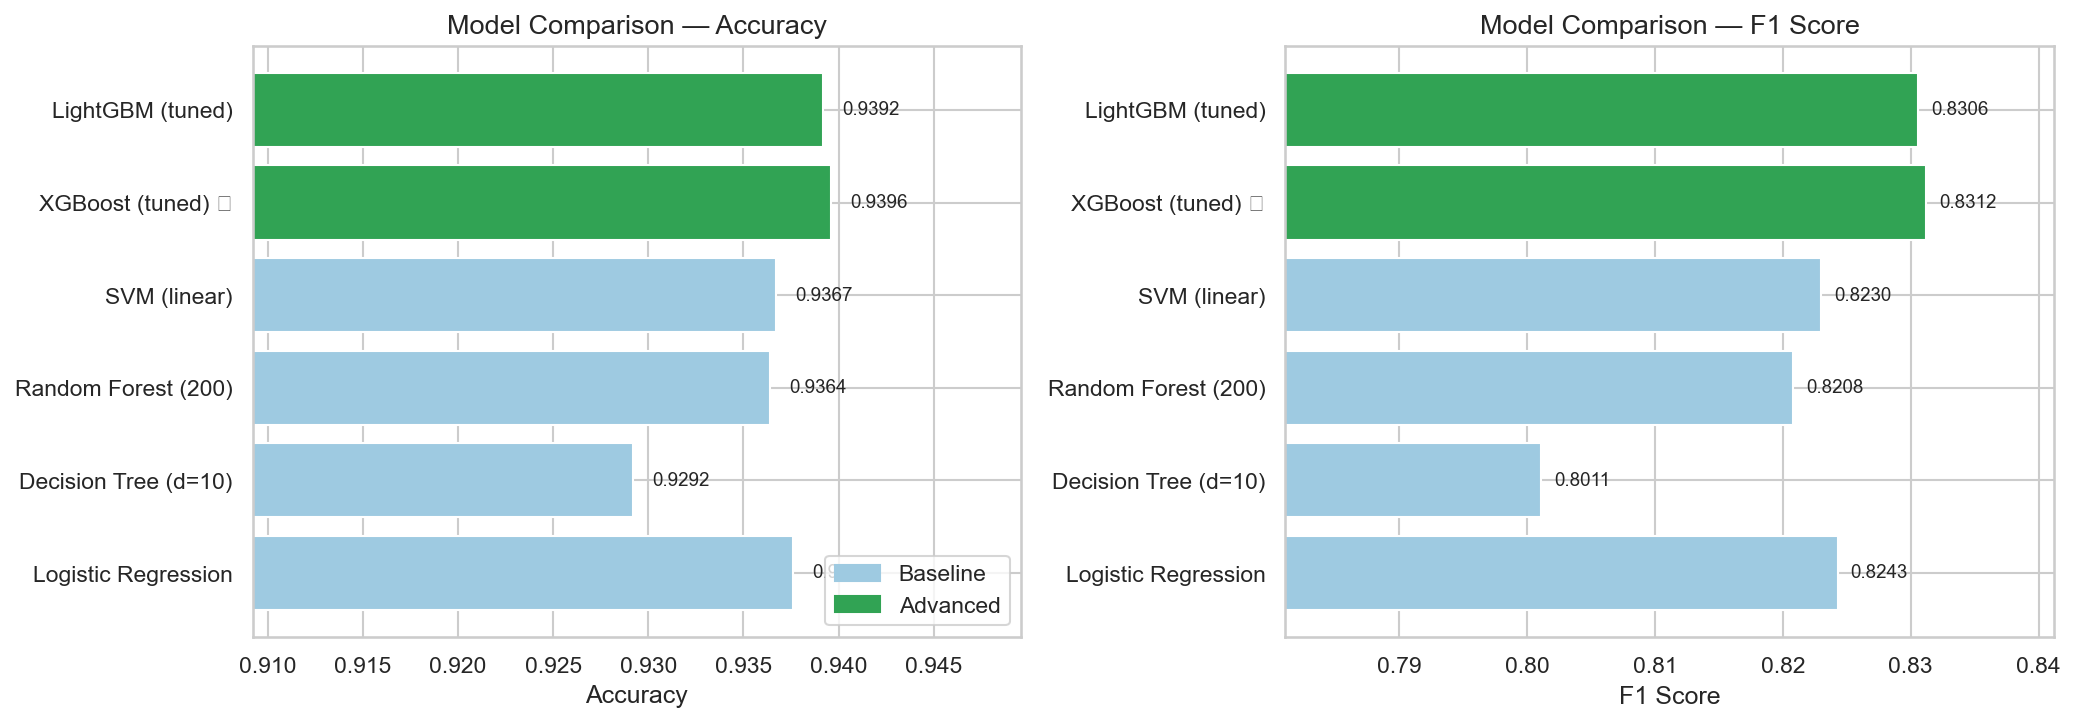
\includegraphics[width=0.95\textwidth]{evaluation/model_comparison.png}
\caption{So sánh Accuracy (trái) và F1-score (phải) giữa các mô hình Baseline và Advanced}
\label{fig:model_comparison}
\end{figure}

\textbf{Nhận xét}: XGBoost (tuned) đạt Accuracy cao nhất (93,96\%) và F1-score cao nhất (0,8312). Tuy nhiên, sự chênh lệch giữa các mô hình tương đối nhỏ ($< 1\%$ Accuracy giữa Baseline và Advanced). Có ba nguyên nhân chính giải thích điều này:

\begin{itemize}[noitemsep]
    \item \textbf{Feature Engineering chất lượng cao}: Bước tạo đặc trưng tương tác (Mục~\ref{subsec:interaction_features}) và Age Binning đã ``giúp sẵn'' các mô hình đơn giản nắm bắt được các pattern phi tuyến --- giảm lợi thế vốn có của mô hình phức tạp.
    \item \textbf{Đặc tính dữ liệu}: Bộ dữ liệu synthetic có cấu trúc tương đối sạch và pattern rõ ràng (Age là đặc trưng chi phối, $r = -0{,}565$), khiến ngay cả mô hình tuyến tính cũng phân tách tốt.
    \item \textbf{Manual Tuning bảo thủ}: Phương pháp tuning thủ công không khai thác triệt để không gian siêu tham số như Grid Search hay Bayesian Optimization, dẫn đến mô hình nâng cao chưa đạt tiềm năng tối đa. Tuy nhiên, điều này cũng giúp tránh overfitting.
\end{itemize}

Dù chênh lệch Accuracy nhỏ, XGBoost vẫn cải thiện đáng kể ở F1-score (+1,0\% so với Logistic Regression), cho thấy khả năng phân loại lớp thiểu số (Depression = 1) tốt hơn.


\subsection{Confusion Matrix}
\label{subsec:confusion_matrix}

Ma trận nhầm lẫn (\textit{Confusion Matrix}) có cấu trúc tổng quát:

\begin{equation}
\text{Confusion Matrix} = \begin{bmatrix} TN & FP \\ FN & TP \end{bmatrix}
\label{eq:cm}
\end{equation}

Hình~\ref{fig:confusion_matrix} trình bày Confusion Matrix của mô hình XGBoost trên toàn bộ tập huấn luyện (OOF predictions --- Out-of-Fold, tức dự đoán trên validation fold trong quá trình Cross-Validation):

\begin{figure}[H]
\centering
{\setlength{\fboxsep}{3pt}\setlength{\fboxrule}{0.4pt}%
\fbox{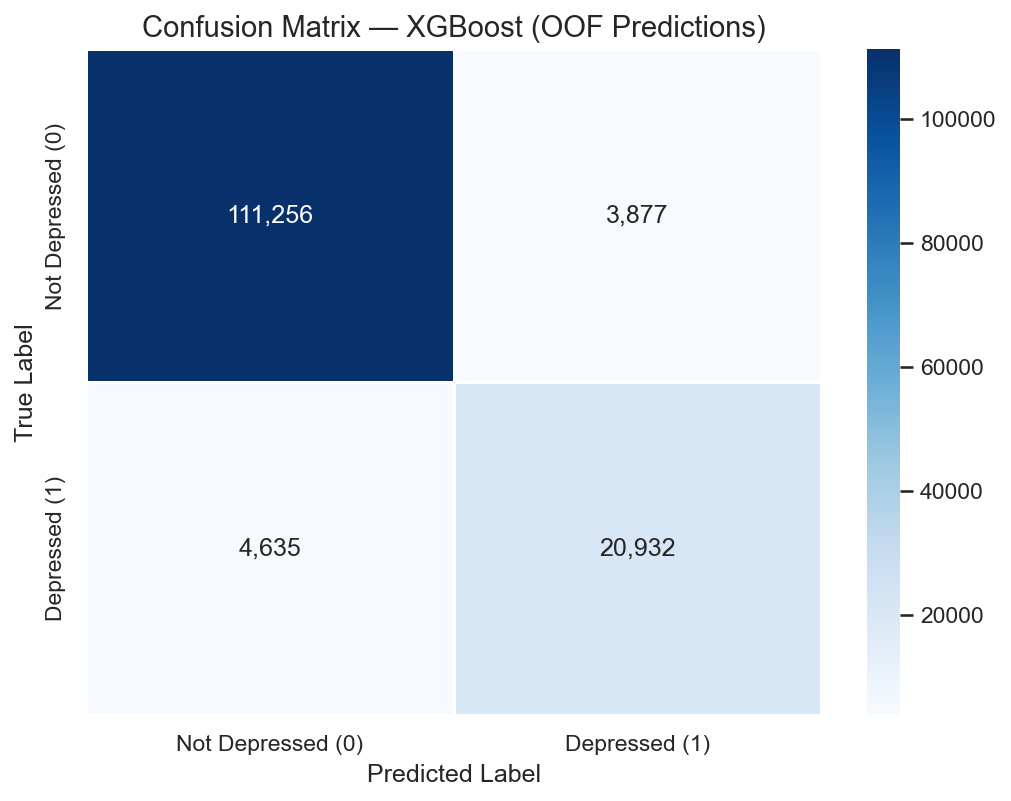
\includegraphics[width=0.58\textwidth]{evaluation/confusion_matrix.png}}}
\caption{Confusion Matrix --- XGBoost (OOF Predictions)}
\label{fig:confusion_matrix}
\end{figure}

\textbf{Phân tích chi tiết}:
\begin{itemize}[noitemsep]
    \item $TN = 111.256$: 96,6\% mẫu không trầm cảm được dự đoán đúng.
    \item $TP = 20.932$: 81,9\% mẫu trầm cảm được phát hiện chính xác.
    \item $FP = 3.877$: 3,4\% mẫu không trầm cảm bị dự đoán nhầm là trầm cảm (\textit{false alarm}).
    \item $FN = 4.635$: 18,1\% mẫu trầm cảm bị bỏ sót --- đây là con số \textbf{đáng lo ngại nhất} trong bài toán y tế, vì bỏ sót người bệnh có thể dẫn đến hậu quả nghiêm trọng.
\end{itemize}

\subsection{Classification Report}
\label{subsec:classification_report}

Bảng~\ref{tab:classification_report} trình bày báo cáo phân loại chi tiết cho từng lớp:

\begin{table}[H]
\centering
\caption{Classification Report --- XGBoost (OOF)}
\label{tab:classification_report}
\begin{tabular}{lcccc}
\toprule
\textbf{Lớp} & \textbf{Precision} & \textbf{Recall} & \textbf{F1-score} & \textbf{Support} \\
\midrule
0 (Không trầm cảm) & 0,9600 & 0,9663 & 0,9632 & 115.133 \\
1 (Trầm cảm) & 0,8437 & 0,8187 & 0,8310 & 25.567 \\
\midrule
\textbf{Accuracy} & \multicolumn{4}{c}{\textbf{0,9395}} \\
Macro avg & 0,9019 & 0,8925 & 0,8971 & 140.700 \\
Weighted avg & 0,9389 & 0,9395 & 0,9391 & 140.700 \\
\bottomrule
\end{tabular}
\end{table}

\textbf{Phân tích trade-off Precision vs Recall}: Đối với lớp 1 (Trầm cảm), Recall = 0,819 cho thấy mô hình phát hiện được ~82\% ca trầm cảm. Trong bối cảnh sàng lọc sức khỏe tâm thần, việc nâng cao Recall (giảm False Negative) có ý nghĩa quan trọng hơn Precision, vì bỏ sót một ca bệnh nguy hiểm hơn so với cảnh báo nhầm.

\subsection{ROC-AUC Curve}
\label{subsec:roc_auc}

Đường cong ROC (\textit{Receiver Operating Characteristic}) biểu diễn mối quan hệ giữa True Positive Rate (Recall) và False Positive Rate khi thay đổi ngưỡng phân loại. Diện tích dưới đường cong:

\begin{equation}
\text{AUC} = \int_0^1 \text{TPR}(t)\, d\text{FPR}(t)
\label{eq:auc}
\end{equation}

trong đó $\text{TPR}(t) = \frac{TP}{TP + FN}$ và $\text{FPR}(t) = \frac{FP}{FP + TN}$ tại ngưỡng $t$.

\begin{figure}[H]
\centering
{\setlength{\fboxsep}{3pt}\setlength{\fboxrule}{0.4pt}%
\fbox{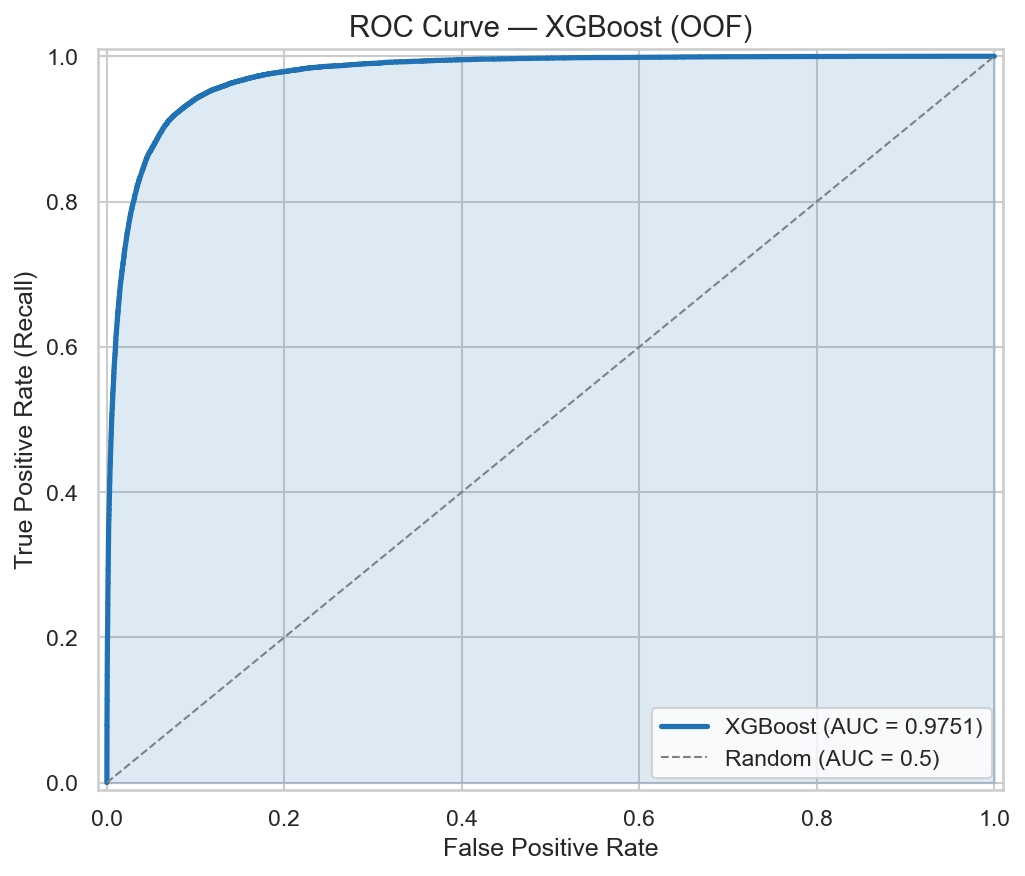
\includegraphics[width=0.58\textwidth]{evaluation/roc_curve.png}}}
\caption{Đường cong ROC --- XGBoost (OOF), AUC = 0,9751}
\label{fig:roc_curve}
\end{figure}

XGBoost đạt \textbf{AUC = 0,9751}, rất gần giá trị tối ưu 1,0. Điều này có nghĩa: khi chọn ngẫu nhiên một mẫu trầm cảm và một mẫu không trầm cảm, mô hình cho mẫu trầm cảm xác suất dự đoán cao hơn mẫu không trầm cảm trong 97,51\% trường hợp. Đường cong nằm rất xa đường chéo (random classifier, AUC = 0,5), xác nhận khả năng phân biệt xuất sắc của mô hình.

\subsection{Feature Importance và SHAP Analysis}
\label{subsec:shap}

\subsubsection{Feature Importance (Built-in)}

Hình~\ref{fig:builtin_fi} so sánh Feature Importance (Gain) giữa XGBoost và LightGBM. Một số quan sát quan trọng:

\begin{itemize}[noitemsep]
    \item \textbf{XGBoost} đặt trọng số cao nhất cho \texttt{age\_group} (0,34) và \texttt{Suicidal Thoughts} (0,22), cho thấy mô hình phụ thuộc mạnh vào nhóm tuổi và yếu tố tâm lý.
    \item \textbf{LightGBM} phân bổ importance đồng đều hơn, với \texttt{Age} đứng đầu. Đặc biệt, LightGBM đánh giá cao các đặc trưng Target Encoded (\texttt{City\_te}, \texttt{Profession\_te}).
    \item Sự khác biệt phản ánh chiến lược growth khác nhau: Level-wise (XGBoost) vs Leaf-wise (LightGBM).
\end{itemize}

\begin{figure}[H]
\centering
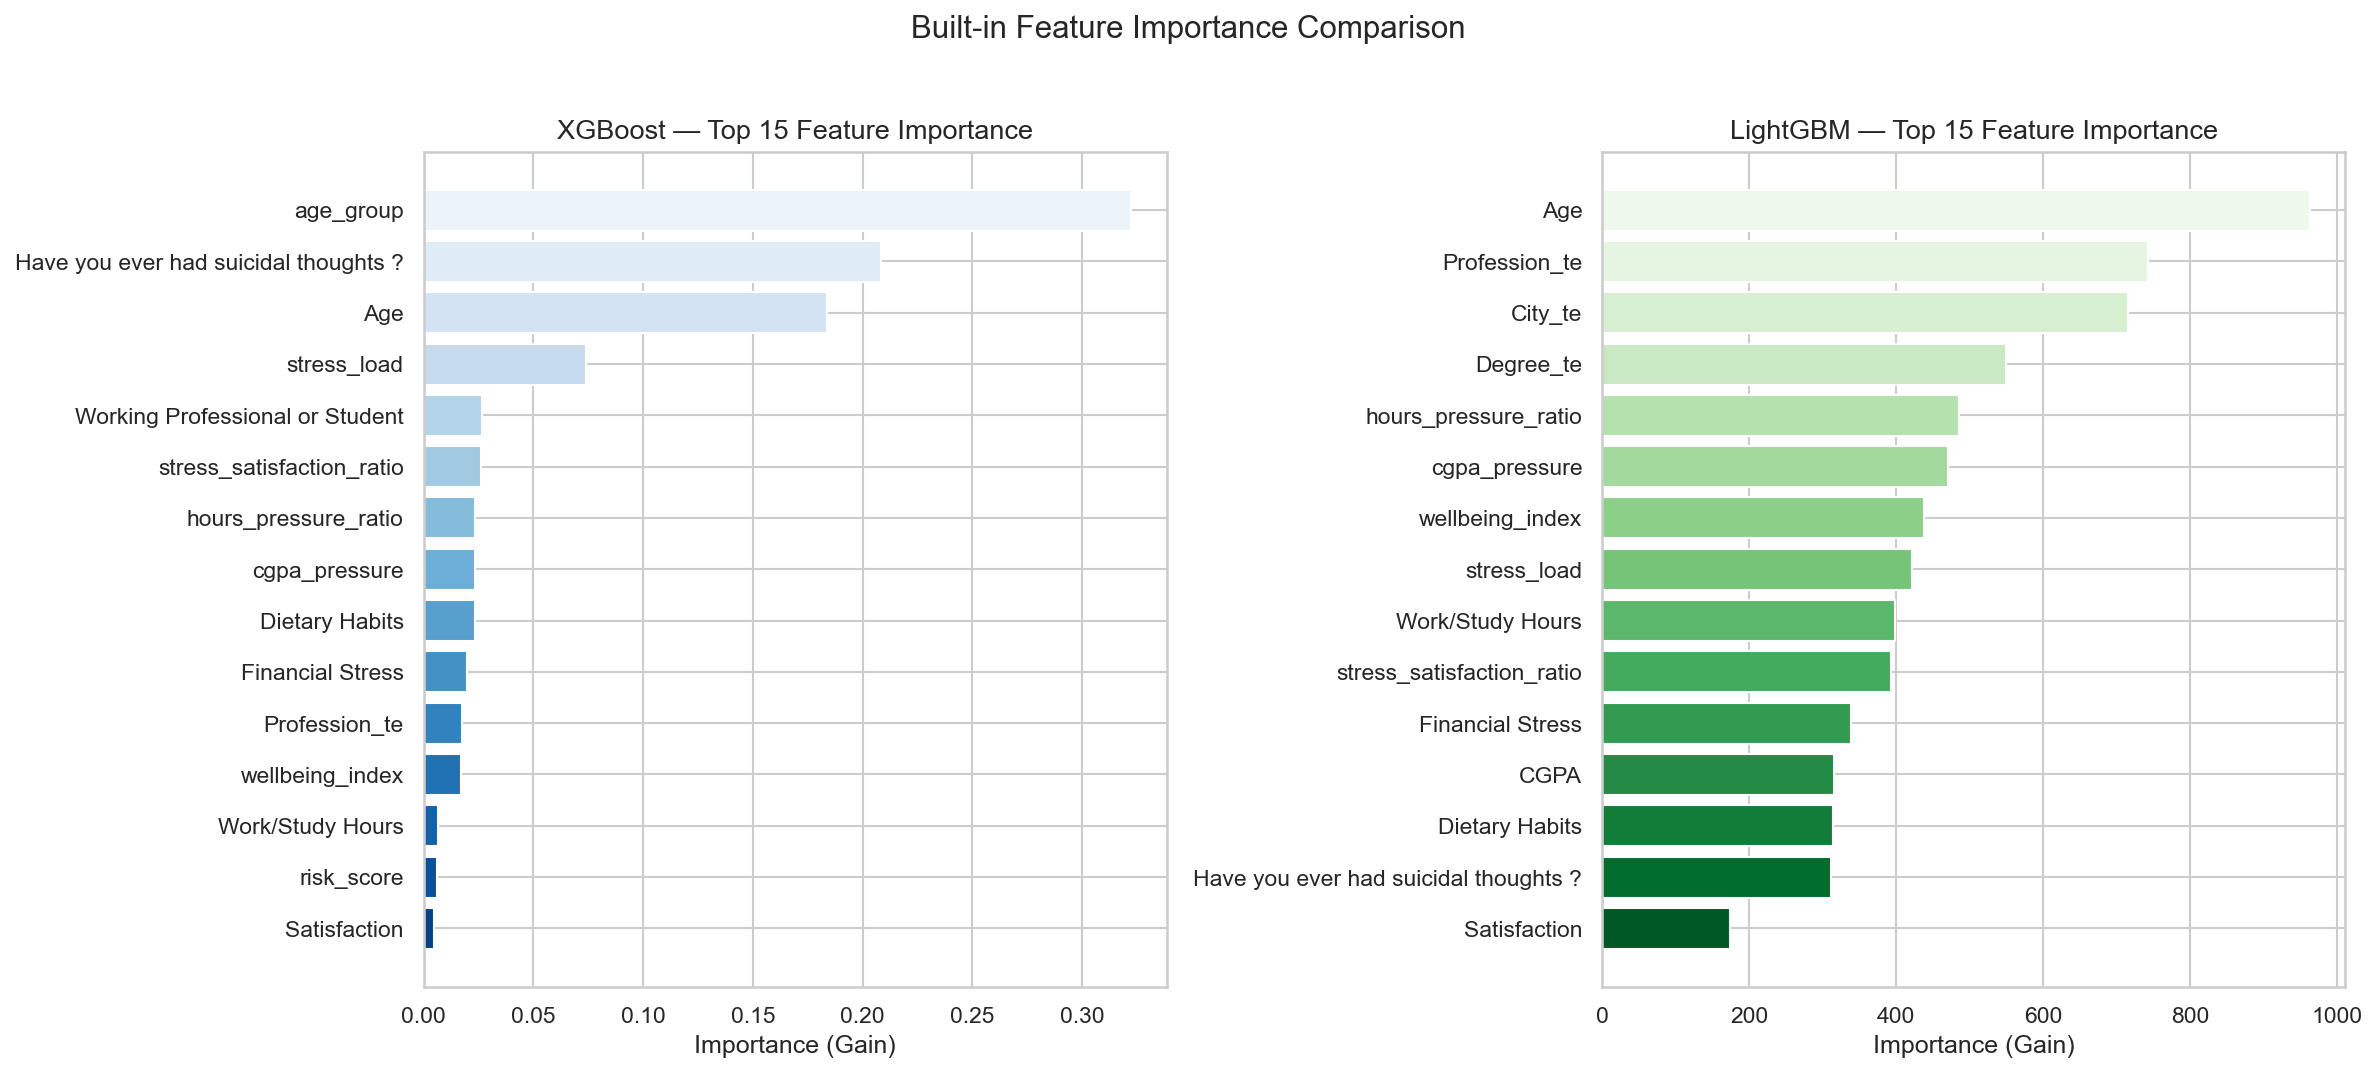
\includegraphics[width=0.95\textwidth]{evaluation/builtin_fi.png}
\caption{So sánh Built-in Feature Importance (Gain): XGBoost (trái) vs LightGBM (phải)}
\label{fig:builtin_fi}
\end{figure}

\subsubsection{SHAP Summary Plot}

SHAP (SHapley Additive exPlanations)~\cite{lundberg2017shap} cung cấp giải thích toàn cục (\textit{global interpretation}) về cách mỗi đặc trưng ảnh hưởng đến dự đoán. Hình~\ref{fig:shap_summary} trình bày SHAP summary plot (dot plot) cho XGBoost:

\begin{figure}[H]
\centering
{\setlength{\fboxsep}{3pt}\setlength{\fboxrule}{0.4pt}%
\fbox{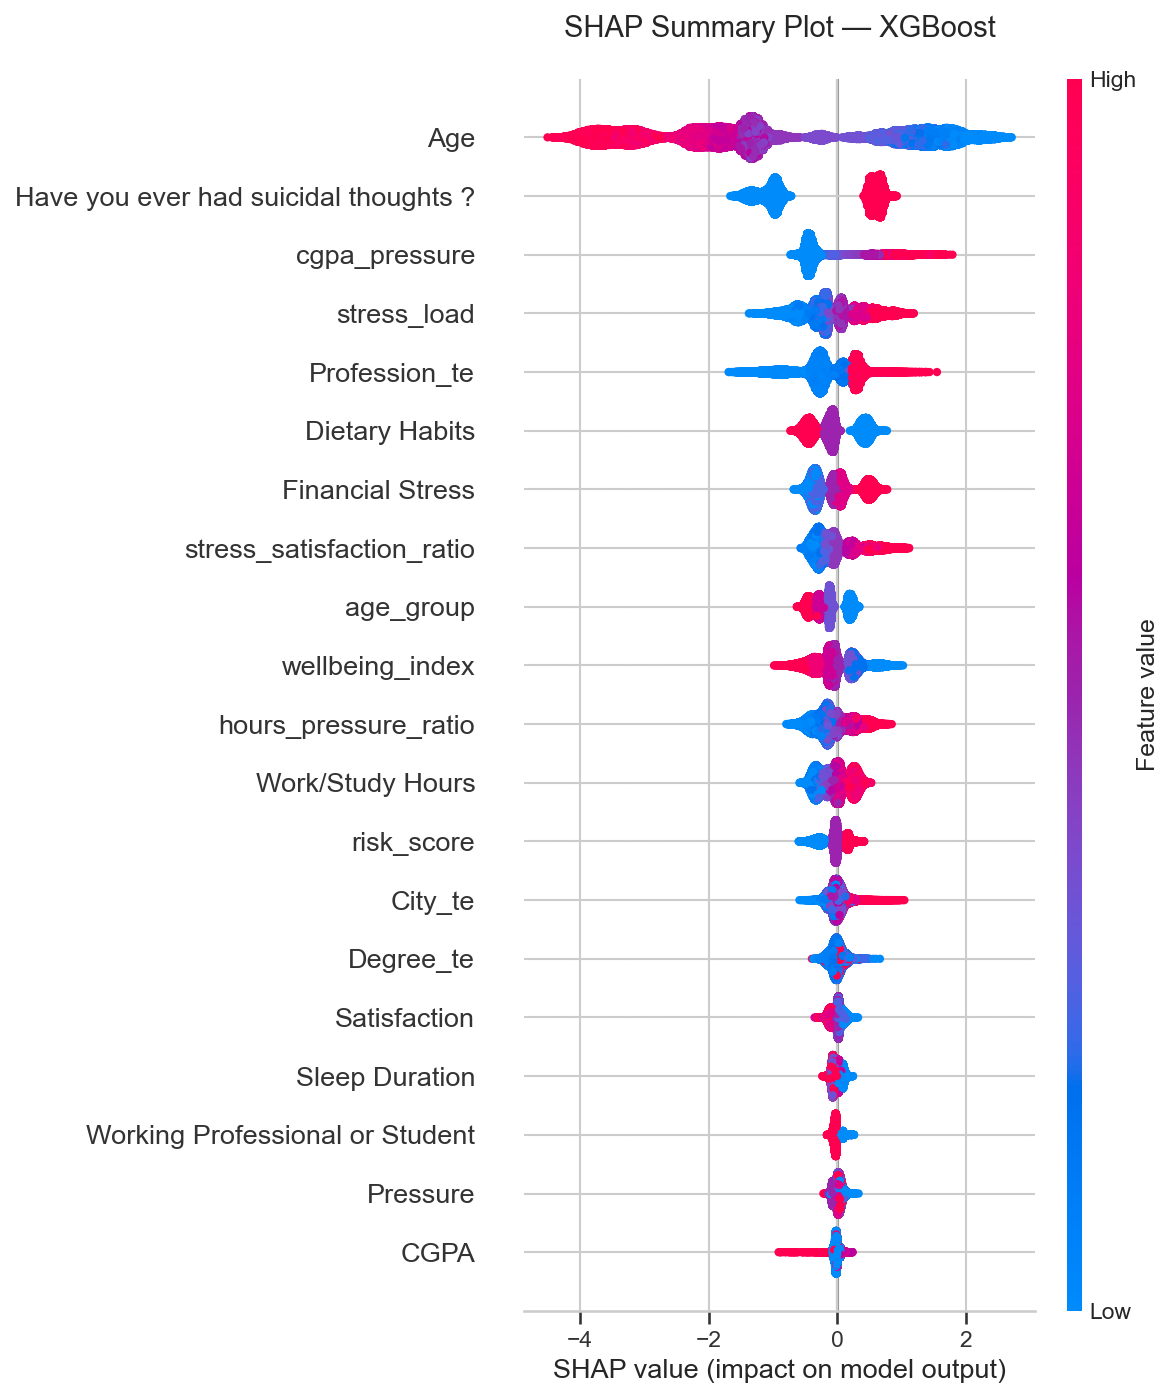
\includegraphics[width=0.63\textwidth]{evaluation/shap_summary.png}}}
\caption{SHAP Summary Plot --- XGBoost: mỗi điểm là một mẫu, màu đỏ = giá trị cao, xanh = giá trị thấp}
\label{fig:shap_summary}
\end{figure}

\textbf{Phân tích chiều tác động}:
\begin{itemize}[noitemsep]
    \item \textbf{Age}: Giá trị thấp (đỏ, bên phải) $\rightarrow$ SHAP dương mạnh $\rightarrow$ \textit{người trẻ có rủi ro trầm cảm cao}. Giá trị cao (xanh, bên trái) $\rightarrow$ SHAP âm lớn $\rightarrow$ \textit{người lớn tuổi có rủi ro thấp}. Đây là pattern rất rõ ràng, phù hợp với kết quả EDA.
    \item \textbf{Suicidal Thoughts}: Giá trị cao (đỏ) $\rightarrow$ SHAP dương mạnh (+0,85 trung bình) $\rightarrow$ \textit{yếu tố rủi ro đáng kể}.
    \item \textbf{cgpa\_pressure}: Giá trị cao $\rightarrow$ SHAP dương $\rightarrow$ \textit{sinh viên có CGPA × áp lực cao có nguy cơ trầm cảm cao hơn}.
    \item \textbf{stress\_load}: Tương tự, căng thẳng tổng hợp cao đẩy dự đoán về phía trầm cảm.
\end{itemize}

\subsubsection{SHAP Bar Plot}

Hình~\ref{fig:shap_bar} xếp hạng các đặc trưng theo giá trị $\text{mean}(|\text{SHAP}|)$, phản ánh mức ảnh hưởng trung bình tuyệt đối lên kết quả dự đoán:

\begin{figure}[H]
\centering
{\setlength{\fboxsep}{3pt}\setlength{\fboxrule}{0.4pt}%
\fbox{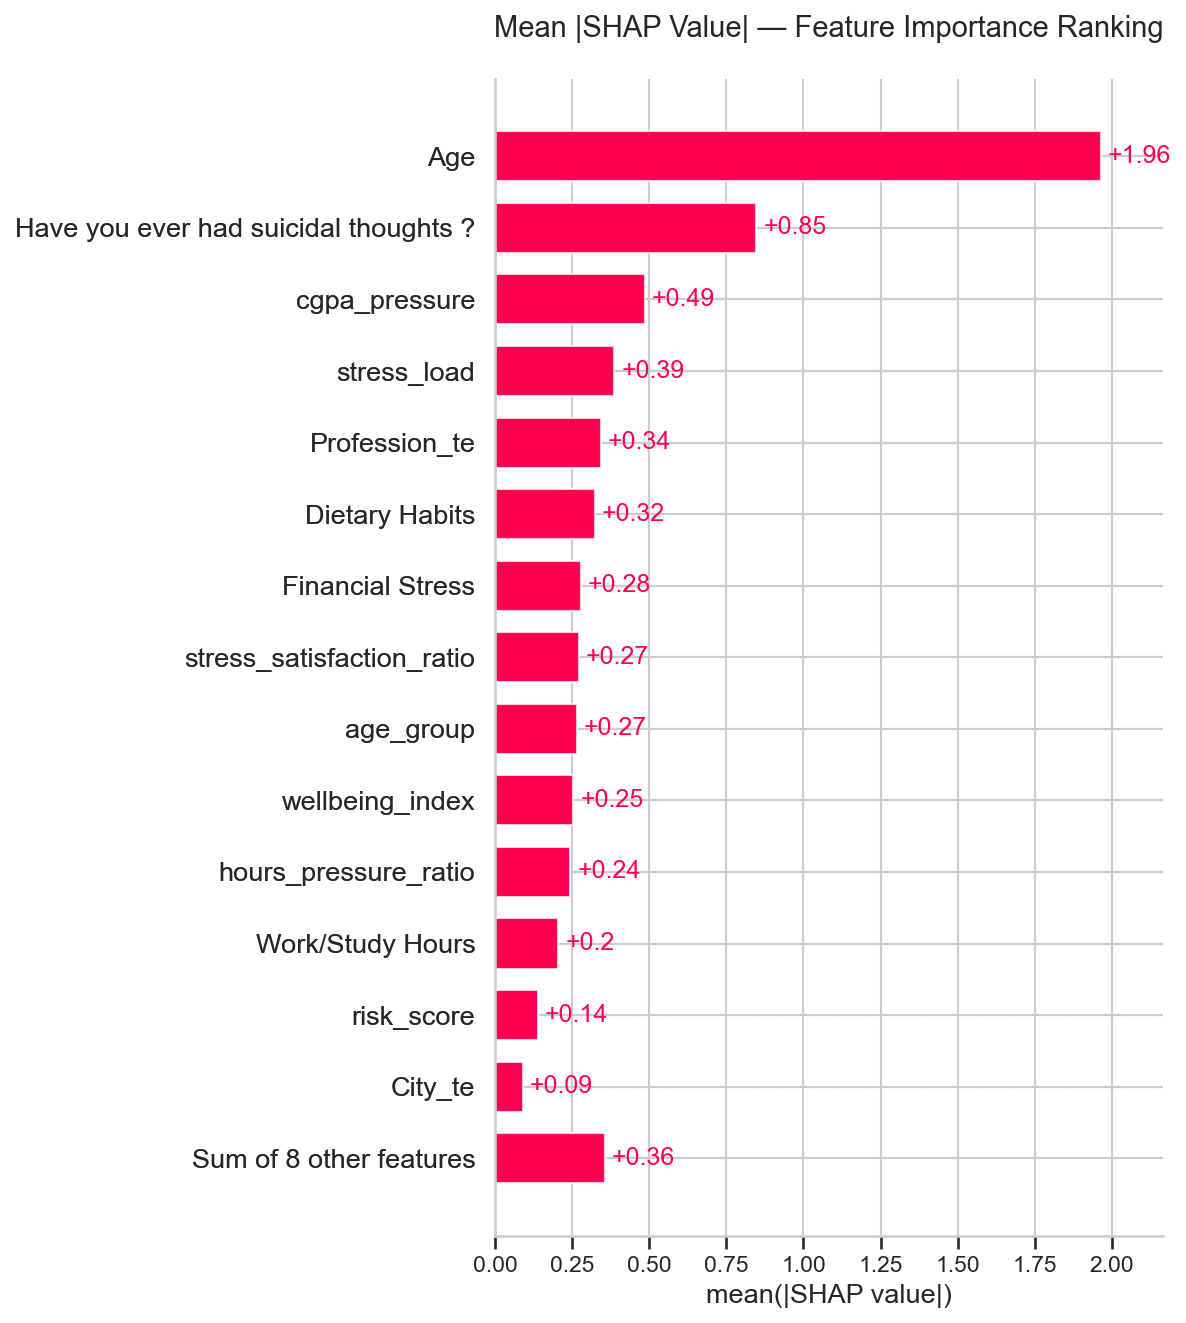
\includegraphics[width=0.63\textwidth]{evaluation/shap_bar.png}}}
\caption{Mean $|\text{SHAP}|$ --- Xếp hạng tầm quan trọng đặc trưng theo SHAP}
\label{fig:shap_bar}
\end{figure}

Top 5 đặc trưng theo SHAP: \texttt{Age} (+1,96), \texttt{Suicidal Thoughts} (+0,85), \texttt{cgpa\_pressure} (+0,49), \texttt{stress\_load} (+0,39), \texttt{Profession\_te} (+0,34). Thứ tự này phần lớn nhất quán với Feature Importance built-in, nhưng SHAP cung cấp thêm thông tin về \textit{chiều tác động} (dương/âm) mà built-in importance không có.

\subsubsection{SHAP Waterfall --- Phân tích ca cụ thể}

Để minh họa khả năng giải thích ở mức \textit{individual prediction}, nhóm chọn hai ca cụ thể:

\textbf{Ca A --- Người bị trầm cảm} (Hình~\ref{fig:waterfall_a}): Đối tượng 26 tuổi, có suy nghĩ tự tử, stress\_load = 20, CGPA = 5,24. Mô hình dự đoán xác suất trầm cảm $P = 0,975$ (rất cao). Các yếu tố đóng góp lớn nhất: Age = 26 (+1,16), Suicidal Thoughts = 1 (+0,63), stress\_load = 20 (+0,59). Tất cả các đặc trưng đều đẩy dự đoán theo hướng ``trầm cảm'', phù hợp với profile lâm sàng của một thanh niên có nhiều yếu tố rủi ro.

\begin{figure}[H]
\centering
{\setlength{\fboxsep}{3pt}\setlength{\fboxrule}{0.4pt}%
\fbox{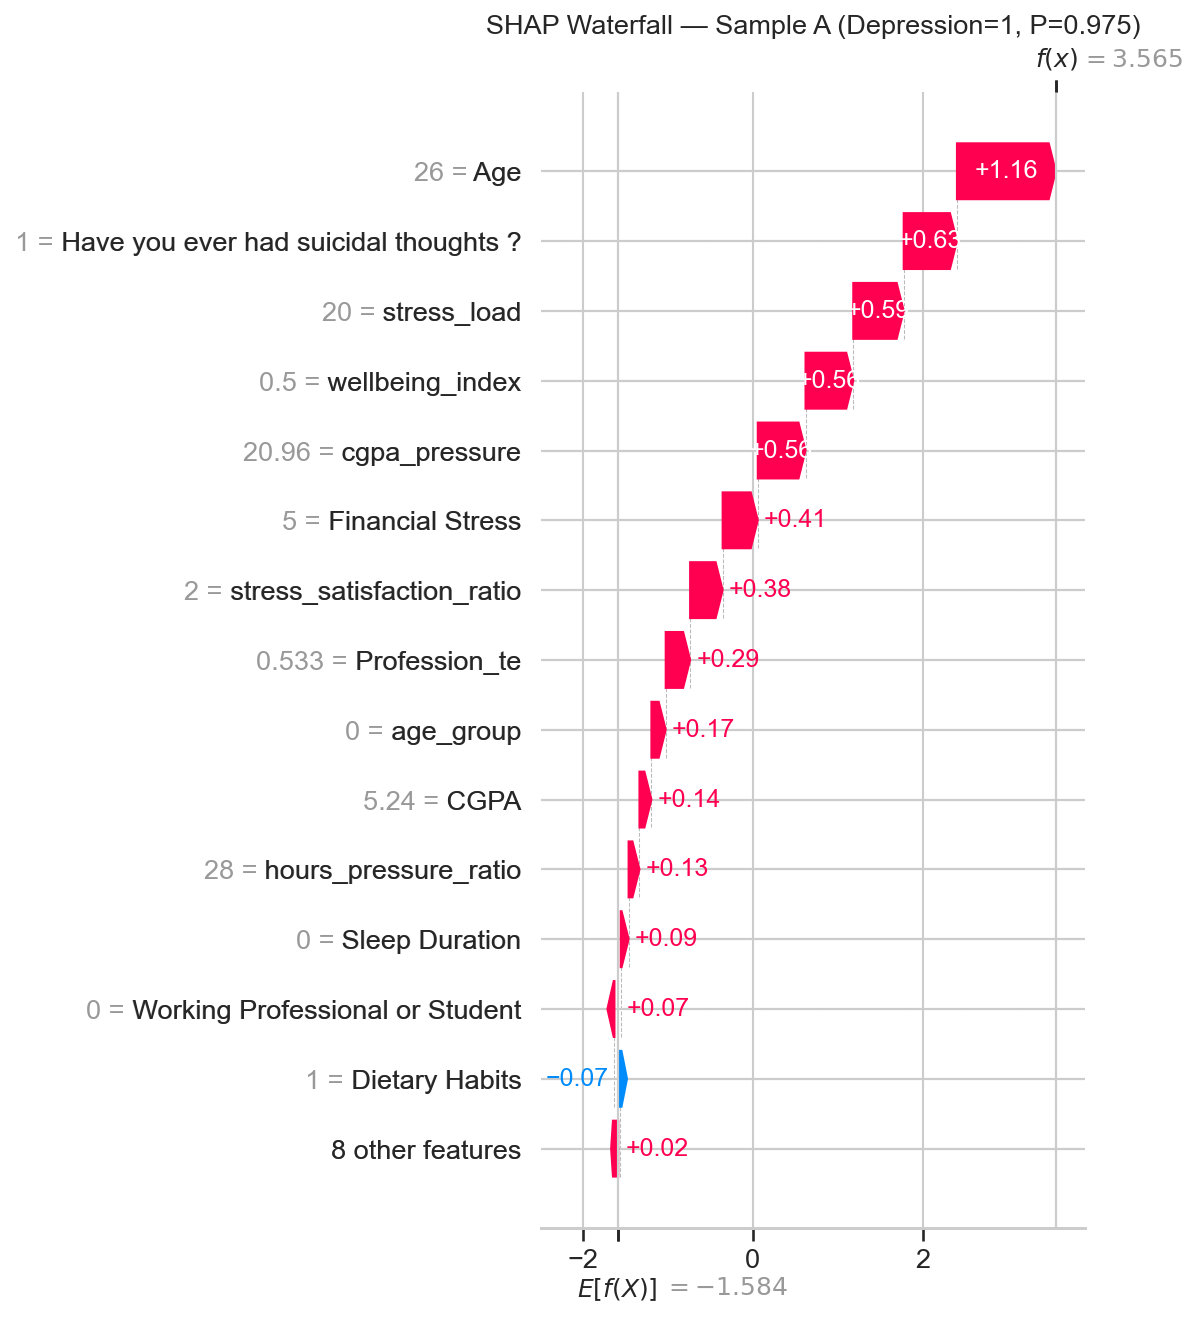
\includegraphics[width=0.58\textwidth]{evaluation/waterfall_a.png}}}
\caption{SHAP Waterfall --- Ca A: Đối tượng trầm cảm (26 tuổi, $P = 0,975$)}
\label{fig:waterfall_a}
\end{figure}

\textbf{Ca B --- Người không bị trầm cảm} (Hình~\ref{fig:waterfall_b}): Đối tượng 59 tuổi, stress\_load = 4, wellbeing\_index = 3,5. Mô hình dự đoán $P = 0,000$ (rất thấp). Yếu tố bảo vệ mạnh nhất: Age = 59 ($-4,0$), Profession\_te ($-1,33$), age\_group = 3 ($-0,46$). Mặc dù có suy nghĩ tự tử (+0,52) và hours\_pressure\_ratio cao (+0,41), tuổi lớn và mức stress thấp đã ``trung hòa'' hoàn toàn các yếu tố rủi ro.

\begin{figure}[H]
\centering
{\setlength{\fboxsep}{3pt}\setlength{\fboxrule}{0.4pt}%
\fbox{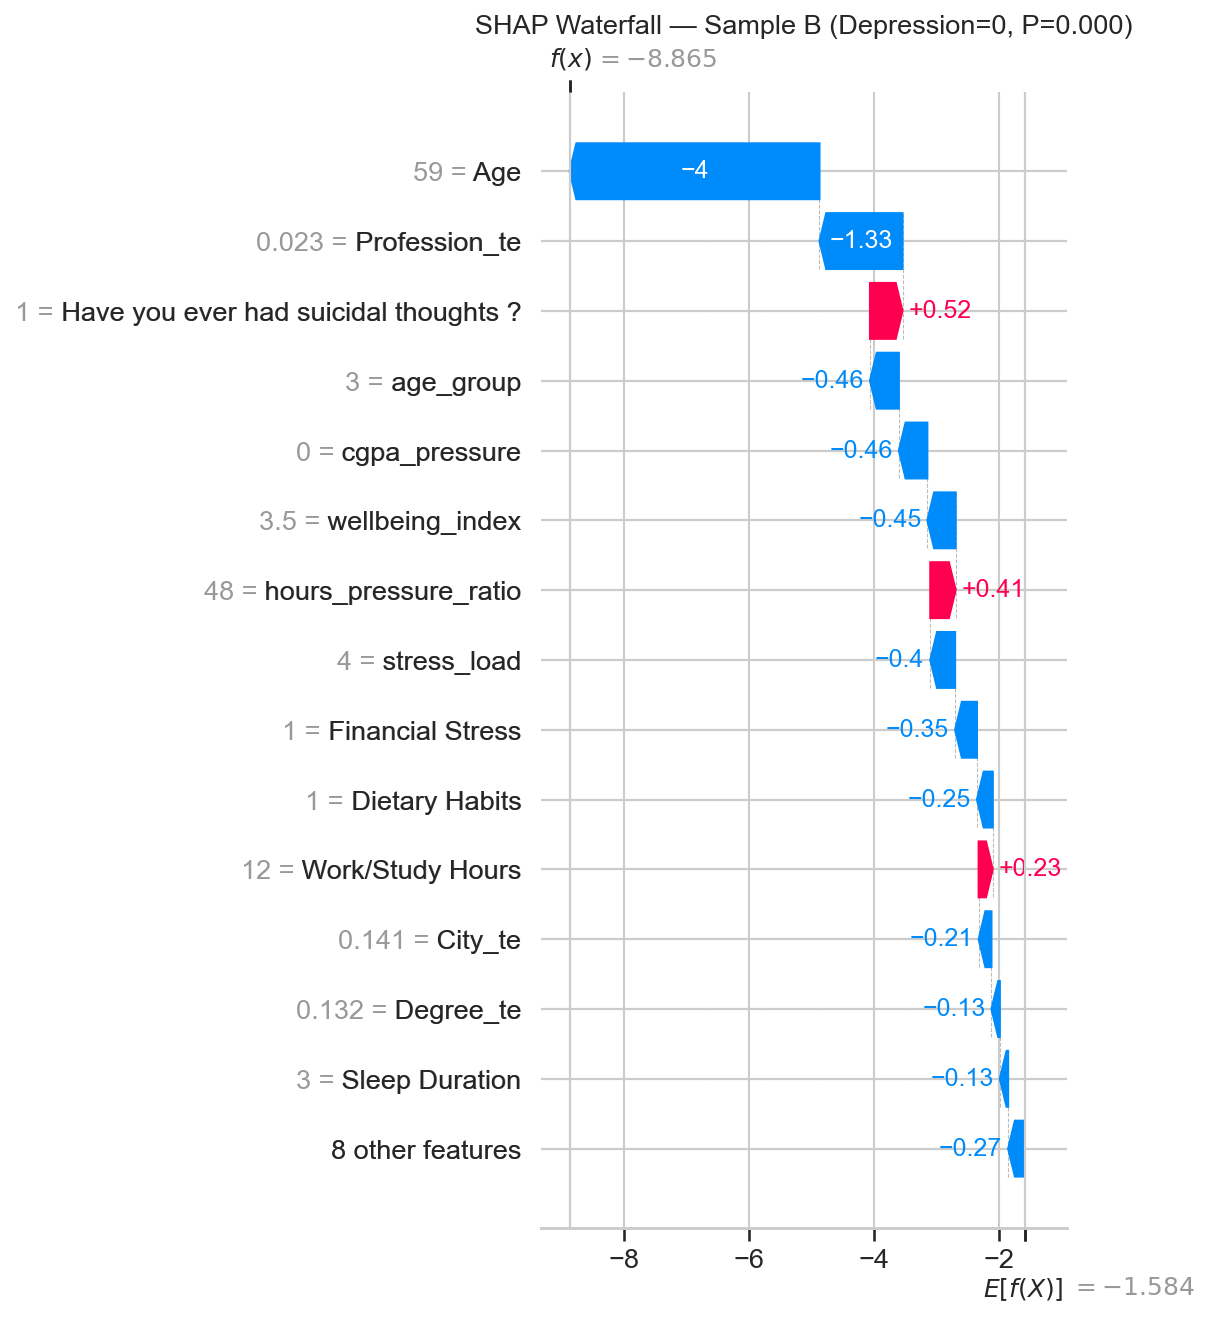
\includegraphics[width=0.58\textwidth]{evaluation/waterfall_b.png}}}
\caption{SHAP Waterfall --- Ca B: Đối tượng không trầm cảm (59 tuổi, $P = 0,000$)}
\label{fig:waterfall_b}
\end{figure}

Hai ca trên cho thấy mô hình XGBoost không chỉ đạt hiệu suất cao mà còn có khả năng \textbf{giải thích được} (\textit{interpretable}), với logic phù hợp với kiến thức lâm sàng về sức khỏe tâm thần.

\subsection{Dự đoán trên tập kiểm tra và Submission}
\label{subsec:submission}

Mô hình XGBoost (best model) được sử dụng để dự đoán trên toàn bộ 93.800 mẫu của tập kiểm tra. Quy trình end-to-end bao gồm: tiền xử lý dữ liệu test (cùng pipeline với train) $\rightarrow$ Feature Engineering $\rightarrow$ dự đoán bằng XGBoost $\rightarrow$ tạo file \texttt{submission.csv} theo format Kaggle (\texttt{id}, \texttt{Depression}).

Kết quả submission chứng minh pipeline hoạt động \textbf{ổn định từ đầu đến cuối} trên dữ liệu chưa từng thấy, không gặp lỗi encoding, missing values, hay các vấn đề tương thích.

\subsection{Nhận xét và phân tích tổng hợp}
\label{subsec:analysis}

\begin{enumerate}[noitemsep]
    \item \textbf{Mô hình tốt nhất}: XGBoost (tuned) với Accuracy = 93,96\%, F1 = 0,8312, AUC = 0,9751.
    \item \textbf{Cải thiện từ Advanced Models}: XGBoost cải thiện +0,2\% Accuracy và +1,0\% F1 so với Logistic Regression baseline, cho thấy giá trị của việc sử dụng mô hình phi tuyến.
    \item \textbf{Feature Engineering hiệu quả}: Các đặc trưng mới (\texttt{stress\_load}, \texttt{cgpa\_pressure}, \texttt{age\_group}) đều xuất hiện trong top 10 quan trọng nhất, xác nhận hiệu quả của bước Feature Engineering.
    \item \textbf{Điểm mạnh}: Pipeline hoàn chỉnh, xử lý tốt noisy data và MNAR missing values, mô hình có khả năng giải thích cao nhờ SHAP.
    \item \textbf{Hạn chế}: Dữ liệu synthetic có thể không phản ánh đầy đủ phức tạp của thực tế; chưa thử nghiệm các kỹ thuật xử lý imbalanced data (SMOTE, class weighting).
\end{enumerate}

\section{Kết luận và hướng phát triển}
\label{sec:conclusion}

\subsection{Kết luận}

Trong đồ án này, nhóm đã xây dựng thành công một pipeline hoàn chỉnh cho bài toán dự đoán rủi ro trầm cảm (\textit{Depression Risk Prediction}) dựa trên dữ liệu khảo sát sức khỏe tâm thần từ cuộc thi Kaggle. Các kết quả chính bao gồm:

\begin{enumerate}[noitemsep]
    \item \textbf{Pipeline xử lý dữ liệu toàn diện}: Xây dựng quy trình 6 bước từ khám phá dữ liệu, tiền xử lý (xử lý noisy data, MNAR missing values, merge conditional columns), kỹ thuật đặc trưng (Target Encoding, Age Binning, Interaction Features), đến đánh giá mô hình.
    
    \item \textbf{Hiệu suất cao}: Mô hình XGBoost (tuned) đạt \textbf{Accuracy = 93,96\%}, \textbf{F1-score = 0,8312} và \textbf{AUC = 0,9751} trên 5-Fold Stratified Cross-Validation. Kết quả này vượt trội so với các mô hình baseline (Logistic Regression, Decision Tree, Random Forest, SVM).
    
    \item \textbf{Khám phá tri thức có giá trị}: Phân tích SHAP cho thấy ba yếu tố ảnh hưởng mạnh nhất đến rủi ro trầm cảm là: \textbf{Tuổi} (người trẻ 18--30 có rủi ro cao nhất), \textbf{Suy nghĩ tự tử} (yếu tố cảnh báo mạnh nhất), và \textbf{Áp lực học tập/công việc kết hợp căng thẳng tài chính}. Các phát hiện này phù hợp với kiến thức y học và có thể hỗ trợ công tác sàng lọc sức khỏe tâm thần.
    
    \item \textbf{Khả năng giải thích}: Nhờ SHAP Waterfall, mô hình có thể giải thích lý do dự đoán cho từng cá nhân cụ thể, tăng tính minh bạch và khả năng ứng dụng thực tế.
\end{enumerate}

\subsection{Hướng phát triển}

Dựa trên các hạn chế đã nhận diện, nhóm đề xuất các hướng phát triển trong tương lai:

\begin{enumerate}[noitemsep]
    \item \textbf{Xử lý mất cân bằng dữ liệu}: Thử nghiệm các kỹ thuật như SMOTE (\textit{Synthetic Minority Over-sampling Technique}), ADASYN, hoặc class weighting để cải thiện Recall cho lớp thiểu số (Depression = 1).
    
    \item \textbf{Mô hình Deep Learning}: Khám phá các kiến trúc chuyên biệt cho dữ liệu dạng bảng như TabNet, FT-Transformer, hoặc Multi-Layer Perceptron (MLP) với dropout và batch normalization.
    
    \item \textbf{Ensemble nâng cao}: Kết hợp nhiều mô hình khác nhau (stacking, blending) để tận dụng điểm mạnh của từng mô hình thành phần.
    
    \item \textbf{Thu thập dữ liệu thực tế}: Thay thế dữ liệu synthetic bằng dữ liệu khảo sát thực tế, bổ sung thêm các yếu tố kinh tế -- xã hội, khí hậu, và lịch sử điều trị.
    
    \item \textbf{Triển khai ứng dụng}: Xây dựng ứng dụng web hoặc mobile cho phép nhập thông tin cá nhân và nhận kết quả sàng lọc trầm cảm nhanh, hỗ trợ bác sĩ và chuyên gia tâm lý trong quy trình đánh giá ban đầu.
    
    \item \textbf{Tối ưu ngưỡng phân loại}: Thay vì sử dụng ngưỡng mặc định 0,5, áp dụng threshold tuning dựa trên chi phí sai lầm (\textit{cost-sensitive learning}) để ưu tiên giảm False Negative trong bối cảnh y tế.
\end{enumerate}


% References
\begin{thebibliography}{9}

\bibitem{kaggle2024}
Kaggle, ``Playground Series --- Season 4, Episode 11: Exploring Mental Health Data,'' 2024.
\textit{Available}: \url{https://www.kaggle.com/competitions/playground-series-s4e11}

\bibitem{chen2016xgboost}
T. Chen and C. Guestrin, ``XGBoost: A Scalable Tree Boosting System,'' in \textit{Proceedings of the 22nd ACM SIGKDD International Conference on Knowledge Discovery and Data Mining}, pp. 785--794, 2016.

\bibitem{ke2017lightgbm}
G. Ke, Q. Meng, T. Finley, T. Wang, W. Chen, W. Ma, Q. Ye, and T.-Y. Liu, ``LightGBM: A Highly Efficient Gradient Boosting Decision Tree,'' in \textit{Advances in Neural Information Processing Systems (NeurIPS)}, vol. 30, pp. 3146--3154, 2017.

\bibitem{lundberg2017shap}
S. M. Lundberg and S.-I. Lee, ``A Unified Approach to Interpreting Model Predictions,'' in \textit{Advances in Neural Information Processing Systems (NeurIPS)}, vol. 30, pp. 4765--4774, 2017.

\bibitem{sklearn2011}
F. Pedregosa, G. Varoquaux, A. Gramfort, V. Michel, B. Thirion, O. Grisel, M. Blondel, P. Prettenhofer, R. Weiss, V. Dubourg, J. Vanderplas, A. Passos, D. Cournapeau, M. Brucher, M. Perrot, and E. Duchesnay, ``Scikit-learn: Machine Learning in Python,'' \textit{Journal of Machine Learning Research}, vol. 12, pp. 2825--2830, 2011.

\bibitem{mckinney2010}
W. McKinney, ``Data Structures for Statistical Computing in Python,'' in \textit{Proceedings of the 9th Python in Science Conference}, pp. 56--61, 2010.

\end{thebibliography}


% Appendix
% \appendix
% \input{appendix/appendix.tex}
\end{document}